% Options for packages loaded elsewhere
% Options for packages loaded elsewhere
\PassOptionsToPackage{unicode}{hyperref}
\PassOptionsToPackage{hyphens}{url}
\PassOptionsToPackage{dvipsnames,svgnames,x11names}{xcolor}
%
\documentclass[
  11pt,
  letterpaper,
]{article}
\usepackage{xcolor}
\usepackage[margin=1in]{geometry}
\usepackage{amsmath,amssymb}
\setcounter{secnumdepth}{5}
\usepackage{iftex}
\ifPDFTeX
  \usepackage[T1]{fontenc}
  % \usepackage[utf8]{inputenc}
  \usepackage{textcomp} % provide euro and other symbols
\else % if luatex or xetex
  \usepackage{unicode-math} % this also loads fontspec
  \defaultfontfeatures{Scale=MatchLowercase}
  \defaultfontfeatures[\rmfamily]{Ligatures=TeX,Scale=1}
\fi
\usepackage{lmodern}
\ifPDFTeX\else
  % xetex/luatex font selection
\fi
% Use upquote if available, for straight quotes in verbatim environments
\IfFileExists{upquote.sty}{\usepackage{upquote}}{}
\IfFileExists{microtype.sty}{% use microtype if available
  \usepackage[]{microtype}
  \UseMicrotypeSet[protrusion]{basicmath} % disable protrusion for tt fonts
}{}
\makeatletter
\@ifundefined{KOMAClassName}{% if non-KOMA class
  \IfFileExists{parskip.sty}{%
    \usepackage{parskip}
  }{% else
    \setlength{\parindent}{0pt}
    \setlength{\parskip}{6pt plus 2pt minus 1pt}}
}{% if KOMA class
  \KOMAoptions{parskip=half}}
\makeatother
% Make \paragraph and \subparagraph free-standing
\makeatletter
\ifx\paragraph\undefined\else
  \let\oldparagraph\paragraph
  \renewcommand{\paragraph}{
    \@ifstar
      \xxxParagraphStar
      \xxxParagraphNoStar
  }
  \newcommand{\xxxParagraphStar}[1]{\oldparagraph*{#1}\mbox{}}
  \newcommand{\xxxParagraphNoStar}[1]{\oldparagraph{#1}\mbox{}}
\fi
\ifx\subparagraph\undefined\else
  \let\oldsubparagraph\subparagraph
  \renewcommand{\subparagraph}{
    \@ifstar
      \xxxSubParagraphStar
      \xxxSubParagraphNoStar
  }
  \newcommand{\xxxSubParagraphStar}[1]{\oldsubparagraph*{#1}\mbox{}}
  \newcommand{\xxxSubParagraphNoStar}[1]{\oldsubparagraph{#1}\mbox{}}
\fi
\makeatother


\usepackage{longtable,booktabs,array}
\newcounter{none} % for unnumbered tables
\usepackage{calc} % for calculating minipage widths
% Correct order of tables after \paragraph or \subparagraph
\usepackage{etoolbox}
\makeatletter
\patchcmd\longtable{\par}{\if@noskipsec\mbox{}\fi\par}{}{}
\makeatother
% Allow footnotes in longtable head/foot
\IfFileExists{footnotehyper.sty}{\usepackage{footnotehyper}}{\usepackage{footnote}}
\makesavenoteenv{longtable}
\usepackage{graphicx}
\makeatletter
\newsavebox\pandoc@box
\newcommand*\pandocbounded[1]{% scales image to fit in text height/width
  \sbox\pandoc@box{#1}%
  \Gscale@div\@tempa{\textheight}{\dimexpr\ht\pandoc@box+\dp\pandoc@box\relax}%
  \Gscale@div\@tempb{\linewidth}{\wd\pandoc@box}%
  \ifdim\@tempb\p@<\@tempa\p@\let\@tempa\@tempb\fi% select the smaller of both
  \ifdim\@tempa\p@<\p@\scalebox{\@tempa}{\usebox\pandoc@box}%
  \else\usebox{\pandoc@box}%
  \fi%
}
% Set default figure placement to htbp
\def\fps@figure{htbp}
\makeatother


% definitions for citeproc citations
\NewDocumentCommand\citeproctext{}{}
\NewDocumentCommand\citeproc{mm}{%
  \begingroup\def\citeproctext{#2}\cite{#1}\endgroup}
\makeatletter
 % allow citations to break across lines
 \let\@cite@ofmt\@firstofone
 % avoid brackets around text for \cite:
 \def\@biblabel#1{}
 \def\@cite#1#2{{#1\if@tempswa , #2\fi}}
\makeatother
\newlength{\cslhangindent}
\setlength{\cslhangindent}{1.5em}
\newlength{\csllabelwidth}
\setlength{\csllabelwidth}{3em}
\newenvironment{CSLReferences}[2] % #1 hanging-indent, #2 entry-spacing
 {\begin{list}{}{%
  \setlength{\itemindent}{0pt}
  \setlength{\leftmargin}{0pt}
  \setlength{\parsep}{0pt}
  % turn on hanging indent if param 1 is 1
  \ifodd #1
   \setlength{\leftmargin}{\cslhangindent}
   \setlength{\itemindent}{-1\cslhangindent}
  \fi
  % set entry spacing
  \setlength{\itemsep}{#2\baselineskip}}}
 {\end{list}}
\usepackage{calc}
\newcommand{\CSLBlock}[1]{\hfill\break\parbox[t]{\linewidth}{\strut\ignorespaces#1\strut}}
\newcommand{\CSLLeftMargin}[1]{\parbox[t]{\csllabelwidth}{\strut#1\strut}}
\newcommand{\CSLRightInline}[1]{\parbox[t]{\linewidth - \csllabelwidth}{\strut#1\strut}}
\newcommand{\CSLIndent}[1]{\hspace{\cslhangindent}#1}



\setlength{\emergencystretch}{3em} % prevent overfull lines

\providecommand{\tightlist}{%
  \setlength{\itemsep}{0pt}\setlength{\parskip}{0pt}}



 


\DeclareUnicodeCharacter{2212}{\ensuremath{-}}
\DeclareUnicodeCharacter{2013}{--}
\DeclareUnicodeCharacter{2014}{---}
\DeclareUnicodeCharacter{2009}{\,}
\DeclareUnicodeCharacter{00A0}{~}
\DeclareUnicodeCharacter{00D7}{\ensuremath{\times}}
\DeclareUnicodeCharacter{2264}{\ensuremath{\leq}}
\DeclareUnicodeCharacter{2265}{\ensuremath{\geq}}
\DeclareUnicodeCharacter{2260}{\ensuremath{\neq}}
\DeclareUnicodeCharacter{2248}{\ensuremath{\approx}}
\DeclareUnicodeCharacter{03B1}{\ensuremath{\alpha}}
\DeclareUnicodeCharacter{03B2}{\ensuremath{\beta}}
\DeclareUnicodeCharacter{03C3}{\ensuremath{\sigma}}
\DeclareUnicodeCharacter{03C7}{\ensuremath{\chi}}
\DeclareUnicodeCharacter{2032}{\ensuremath{'}}

\usepackage{caption}
\captionsetup{labelsep=period}

\setcitestyle{round}

% \AtBeginEnvironment{table}{\footnotesize}
\AtBeginEnvironment{apptbl}{\footnotesize}
% Table font size: \footnotesize by default; table-size.lua emits \nexttablesize{\scriptsize}
% before a table whose div has size="scriptsize", which applies to that table only
\makeatletter
\newcommand\table@defaultsize{\footnotesize}
\let\table@size\table@defaultsize
\newcommand\nexttablesize[1]{\gdef\table@size{#1}}
\AtBeginEnvironment{longtable}{\table@size\global\let\table@size\table@defaultsize}
\makeatother

% Figure notes: note-in-float.lua wraps a figure's Note in \floatnote{...}, which
% prints it after the caption (the float package always sets the caption last)
\makeatletter
\let\floatnote@text\@empty
\newcommand\floatnote[1]{\gdef\floatnote@text{#1}}
\newcommand\fs@plainnote{\fs@plain
  \def\@fs@post{\ifx\floatnote@text\@empty\else
    \vspace\abovecaptionskip\noindent\floatnote@text\par
    \global\let\floatnote@text\@empty\fi}}
\makeatother

% Pin appendix floats in place so they stay next to their Note paragraphs
% (deferred inside \AtBeginDocument because Quarto's \newfloat comes after this file)
\AtBeginDocument{%
  \floatstyle{plainnote}\restylefloat{appfig}%
  \floatplacement{appfig}{H}\floatplacement{apptbl}{H}}

% Caption label for appendix tables typeset as breakable longtables (breakable-apptbl.lua);
% position=top restores the skip between the caption and the table's top rule
\AtBeginDocument{\providecommand*\apptblname{Table W}}
\captionsetup[apptbl]{position=top}

% ACL-style title block: bold title; one column per author (bold name, regular
% affiliation, small monospace email)
\makeatletter
\renewcommand\@maketitle{%
  \newpage\null\vskip 0.5em
  \begin{center}
    {\Large\bfseries \@title\par}
    \vskip 1.5em
    {\normalsize \@author\par}
  \end{center}
  \par\vskip 1em}
\newcommand\aclauthor[3]{% name, affiliation lines, email
  \begin{tabular}[t]{@{}c@{}}
    \textbf{#1}\\[1pt]
    #2\\[1pt]
    {\small\texttt{#3}}
  \end{tabular}}
\makeatother

% Hardcoded PDF authors. Runs at \begin{document}, so it overrides the plain
% \author{} Quarto generates from the YAML (the YAML authors still set PDF metadata).
\AtBeginDocument{%
  \author{%
    \aclauthor{Davood Wadi}
      {Desautels Faculty of Management\\ McGill University\\ Montreal, Quebec, Canada}
      {davood.wadi@hec.ca}%
    \hspace{3em}%
    \aclauthor{Yu Ma}
      {Desautels Faculty of Management\\ McGill University\\ Montreal, Quebec, Canada}
      {yu.ma@mcgill.ca}%
  }%
}
\makeatletter
\@ifpackageloaded{float}{}{\usepackage{float}}
\floatstyle{plain}
\@ifundefined{c@chapter}{\newfloat{apptbl}{h}{loapptbl}}{\newfloat{apptbl}{h}{loapptbl}[chapter]}
\floatname{apptbl}{Table W}
\floatstyle{plaintop}
\restylefloat{apptbl}
\newcommand*\quartoapptblref[1]{Table \hyperref[#1]{W\ref{#1}}}
\@ifpackageloaded{caption}{}{\usepackage{caption}}
\DeclareCaptionLabelFormat{quartoapptblreflabelformat}{#1#2}
\captionsetup[apptbl]{labelformat=quartoapptblreflabelformat}
\newcommand*\listofapptbls{\listof{apptbl}{List of Table Ws}}
\makeatother
\makeatletter
\@ifpackageloaded{float}{}{\usepackage{float}}
\floatstyle{plain}
\@ifundefined{c@chapter}{\newfloat{appfig}{h}{loappfig}}{\newfloat{appfig}{h}{loappfig}[chapter]}
\floatname{appfig}{Figure W}
\newcommand*\quartoappfigref[1]{Figure \hyperref[#1]{W\ref{#1}}}
\@ifpackageloaded{caption}{}{\usepackage{caption}}
\DeclareCaptionLabelFormat{quartoappfigreflabelformat}{#1#2}
\captionsetup[appfig]{labelformat=quartoappfigreflabelformat}
\newcommand*\listofappfigs{\listof{appfig}{List of Figure Ws}}
\makeatother
\makeatletter
\@ifpackageloaded{float}{}{\usepackage{float}}
\floatstyle{plain}
\@ifundefined{c@chapter}{\newfloat{appenv}{h}{loapp}}{\newfloat{appenv}{h}{loapp}[chapter]}
\floatname{appenv}{Web Appendix}
\floatstyle{plaintop}
\restylefloat{appenv}
\newcommand*\quartoappref[1]{Web \hyperref[#1]{Appendix\ref{#1}}}
\@ifpackageloaded{caption}{}{\usepackage{caption}}
\DeclareCaptionLabelFormat{quartoappreflabelformat}{#1#2}
\captionsetup[appenv]{labelformat=quartoappreflabelformat}
\newcommand*\listofappenvs{\listof{appenv}{List of Web Appendixs}}
\makeatother
\makeatletter
\@ifpackageloaded{tcolorbox}{}{\usepackage[skins,breakable]{tcolorbox}}
\@ifpackageloaded{fontawesome5}{}{\usepackage{fontawesome5}}
\definecolor{quarto-callout-color}{HTML}{909090}
\definecolor{quarto-callout-note-color}{HTML}{0758E5}
\definecolor{quarto-callout-important-color}{HTML}{CC1914}
\definecolor{quarto-callout-warning-color}{HTML}{EB9113}
\definecolor{quarto-callout-tip-color}{HTML}{00A047}
\definecolor{quarto-callout-caution-color}{HTML}{FC5300}
\definecolor{quarto-callout-color-frame}{HTML}{acacac}
\definecolor{quarto-callout-note-color-frame}{HTML}{4582ec}
\definecolor{quarto-callout-important-color-frame}{HTML}{d9534f}
\definecolor{quarto-callout-warning-color-frame}{HTML}{f0ad4e}
\definecolor{quarto-callout-tip-color-frame}{HTML}{02b875}
\definecolor{quarto-callout-caution-color-frame}{HTML}{fd7e14}
\makeatother
\makeatletter
\@ifpackageloaded{caption}{}{\usepackage{caption}}
\AtBeginDocument{%
\ifdefined\contentsname
  \renewcommand*\contentsname{Table of contents}
\else
  \newcommand\contentsname{Table of contents}
\fi
\ifdefined\listfigurename
  \renewcommand*\listfigurename{List of Figures}
\else
  \newcommand\listfigurename{List of Figures}
\fi
\ifdefined\listtablename
  \renewcommand*\listtablename{List of Tables}
\else
  \newcommand\listtablename{List of Tables}
\fi
\ifdefined\figurename
  \renewcommand*\figurename{Figure}
\else
  \newcommand\figurename{Figure}
\fi
\ifdefined\tablename
  \renewcommand*\tablename{Table}
\else
  \newcommand\tablename{Table}
\fi
}
\@ifpackageloaded{float}{}{\usepackage{float}}
\floatstyle{ruled}
\@ifundefined{c@chapter}{\newfloat{codelisting}{h}{lop}}{\newfloat{codelisting}{h}{lop}[chapter]}
\floatname{codelisting}{Listing}
\newcommand*\listoflistings{\listof{codelisting}{List of Listings}}
\makeatother
\makeatletter
\makeatother
\makeatletter
\@ifpackageloaded{caption}{}{\usepackage{caption}}
\@ifpackageloaded{subcaption}{}{\usepackage{subcaption}}
\makeatother
\usepackage{bookmark}
\IfFileExists{xurl.sty}{\usepackage{xurl}}{} % add URL line breaks if available
\urlstyle{same}
% fallback for those not using the hyperref driver hyperxmp:
\makeatletter
\@ifundefined{xmpquote}{\newcommand{\xmpquote}[1]{#1}}{}
\makeatother
\hypersetup{
  pdftitle={Training decision models for simulating human respondents},
  pdfauthor={Davood Wadi; Yu Ma},
  colorlinks=true,
  linkcolor={blue},
  filecolor={Maroon},
  citecolor={Blue},
  urlcolor={Blue},
  pdfcreator={LaTeX via pandoc}}


\title{Training decision models for simulating human respondents}
\author{Davood Wadi \and Yu Ma}
\date{}
\begin{document}
\maketitle


\textbf{Abstract.}\\
{[}TODO{]}

\textbf{Keywords.} Decision models, large language models, synthetic
respondents, econometric inference, marketing research

\section{Introduction}\label{sec-intro}

Using foundation models as synthetic respondents to simulate consumer
choices has attracted growing interest in marketing and behavioral
research. In marketing, the primary goal is downstream econometric
inference, such as estimating attribute slopes in conjoint analysis or
recovering causal treatment effects in randomized experiments. Most
studies generate synthetic choice data with off-the-shelf generative
large language models (LLMs), yet substituting these outputs for human
responses severely biases downstream regressions (Goli and Singh 2024,
Leng et al. 2026, Wang et al. 2026). This bias arises because
off-the-shelf LLMs are optimized for deterministic text generation and
safety compliance, which collapses choice uncertainty and triggers
refusals. For instance, on a vaccines conjoint subsample (Kreps et al.
2020), off-the-shelf models incur large ordinary least squares (OLS)
treatment-effect error relative to human respondents (Wang et al. 2026).
Contrary to common expectation, using proprietary models or increasing
reasoning effort can even increase this error
(Figure~\ref{fig-intro-off-the-shelf}). Additionally, generative LLMs
are slow and computationally expensive. Since they produce responses as
tokens, approximating their choice probabilities requires costly
Monte-Carlo sampling.

To overcome the time and computation costs of text generation, we
investigate system one decision models (Deußer et al. 2026, Geuter et
al. 2026, Palmer 2026). Unlike generative LLMs, a decision model
replaces the text-generation head with a scoring layer over candidate
options. Given a respondent persona and choice task, it outputs
normalized choice probabilities in a single forward pass. This
single-pass directly generates the probability distribution of choices,
eliminates Monte Carlo sampling cost and noise, and yields exact
expected OLS treatment effects directly from predicted probabilities.
Despite their architectural advantage, off-the-shelf decision models
still suffer from high error in their OLS estimates
(Figure~\ref{fig-intro-off-the-shelf}). Because these models are
pretrained on single-label objective benchmarks rather than human choice
behavior, they treat disagreement among respondents with the same
persona as classification error (Gao et al. 2026).

In this research, we train decision models by updating their weights on
historical human choice microdata, a procedure we call choice training.
Specifically, we minimize respondent-level cross-entropy (CE), which is
equivalent to conditional maximum likelihood estimation, and test
whether choice training transfers to unseen marketing and behavioral
studies.

\begin{figure}

\centering{

\includegraphics[width=0.9\linewidth,height=\textheight,keepaspectratio]{manuscript-training-assets/fig-intro-off-the-shelf.png}

}

\caption{\label{fig-intro-off-the-shelf}OLS treatment-effect error
across off-the-shelf generative LLMs and decision models}

\vspace{\abovecaptionskip}

\noindent \emph{Note.} Bars report OLS
\(\mathrm{MSE}_\beta \times 10^3\) (Equation~\ref{eq-eval-mse}) across
11 vaccine attribute levels on the 200-respondent Vaccines conjoint
subsample (\(n = 1,000\) choice tasks; Wang et al. 2026). Errors are
measured relative to full-sample human estimates (\(N = 1,971\)
respondents; 9,855 choice tasks).

\end{figure}%

Empirically, we evaluate choice training across three open-weight
decision-model scales (0.8B, 4B, and 9B parameters; Palmer 2026). We
evaluate generalizability of our training on four unseen held-out
studies: a nutrition-labeling trial (Grummon et al. 2025), a vaccine
conjoint (Kreps et al. 2020), a consumer-rights conjoint
(Kantorowicz-Reznichenko et al. 2026), and an AI smartphone conjoint
(Magistro et al. 2026). We show that although scaling to proprietary
models or increasing reasoning effort can worsens OLS MSE, choice
training with respondent-level CE substantially lowers this error on
unseen studies, across model scales.

\section{Literature review}\label{sec-lit}

Early work on synthetic respondents prompted off-the-shelf generative
LLMs with demographic profiles to simulate human answers in political,
economic, and marketing surveys (Argyle et al. 2023, Horton et al. 2023,
Santurkar et al. 2023, Goli and Singh 2024). Although these models often
capture average preference directions, systematic discrepancies from
human populations severely bias downstream econometric estimates
(Santurkar et al. 2023, Wadi and Fredette 2025, Leng et al. 2026, Wang
et al. 2026). Common distortions include mode collapse, attenuated
within-group variance, and prompt sensitivity. In choice-based conjoint
analysis, scaling generative model capability or increasing reasoning
effort can worsen preference-estimation error by inducing overly
deterministic choices (Wang et al. 2026). Recent marketing research
addresses these biases while keeping model weights fixed, relying on
human data from the target study or target individuals. These methods
include post-inference econometric debiasing (Wang et al. 2026), optimal
post-inference reweighting across prompts and checkpoints (Leng et al.
2026), individual digital twins conditioned on hundreds of responses per
person (Toubia et al. 2025), and collaborative AI-human research
workflows (Arora et al. 2025). As Hullman et al. (2026) clarify,
post-inference statistical adjustment secures confirmatory validity, yet
both standalone simulation and statistical adjustment still depend on
how closely the underlying model approximates the target human
population.

A growing literature instead updates LLM weights directly on human
behavioral data, spanning target-study, within-category, and cross-study
regimes. On target-study data, small-sample training fails to reliably
recover regression parameters. Wang et al. (2026) show that training
GPT-4o on 50 target-study conjoint tasks worsens standalone parameter
error. Similarly, Wang et al. (2025) find that small human pilot samples
improve response heterogeneity and belief-action coherence, yet still
fail to reproduce the original study's regression coefficients. Ye et
al. (2025) pair target-study training with post-inference rectification,
but their two-stage procedure still requires labeled human responses
from the target study. In marketing conjoints, Brand et al. (2023) train
GPT-3.5 Turbo on respondent-level choices from a prior study and improve
willingness-to-pay estimates for new attributes within the same category
(e.g., toothpaste or laptops). However, they find no transfer across
categories, as laptop-trained models widen errors and flip attribute
signs on tablets. Outside marketing, large-scale behavioral training
improves out-of-study prediction across cognitive psychology (10 million
choices across 160 experiments; {Binz et al.} 2025), social-science
experiments (2.9 million responses across 210 studies; Kolluri et al.
2025), and public-opinion surveys (Suh et al. 2025, Ku et al. 2026,
Huang et al. 2026). Yet these cross-study efforts rely on massive
multi-hundred-study corpora and autoregressive text generation.
Moreover, they evaluate predictive log-likelihood, marginal
distributions, or cell-level distributional distance rather than
econometric treatment-effect recovery.

A parallel architectural stream avoids the latency and sampling variance
of repeated text generation. Several studies extract next-token
probabilities over option symbols (e.g., A, B, and C) from causal LLMs
({Kadavath et al.} 2022, Wadi et al. 2026), yet symbol-level readouts
remain sensitive to vocabulary and token-frequency priors. Single-pass
System One decision models resolve this sensitivity by replacing text
decoding with a pointer scoring head that evaluates candidate options
directly in representation space (Deußer et al. 2026, Geuter et al.
2026, Palmer 2026). This architecture restricts probability mass
strictly to valid options, eliminates refusals, and yields exact
expected OLS treatment effects in one forward pass with zero Monte Carlo
variance. However, off-the-shelf decision models are pretrained on
single-label objective benchmarks such as mathematics, code, and factual
question answering, causing severe overconfidence on subjective human
choice tasks (Gao et al. 2026).

We connect these three streams by applying pre-inference choice training
to compact single-pass decision models (\texttt{0.8B} to \texttt{9B}
parameters). Using respondent-level cross-entropy on just two historical
choice datasets (54,888 tasks), we evaluate unseen-study OLS
treatment-effect recovery across four unrelated domains and response
formats. Unlike post-inference adjustment (Leng et al. 2026, Wang et al.
2026), target-study training (Ye et al. 2025), or digital twins (Toubia
et al. 2025), choice training requires no human data from the target
study. Unlike within-category conjoint training (Brand et al. 2023), it
transfers across product domains and response formats. Finally, unlike
large-scale generative behavioral models ({Binz et al.} 2025, Kolluri et
al. 2025, Suh et al. 2025), it operates at compact single-pass scale
from two datasets and directly lowers econometric treatment-effect
error.

\section{Methodology}\label{sec-methodology}

\begin{figure}

\centering{

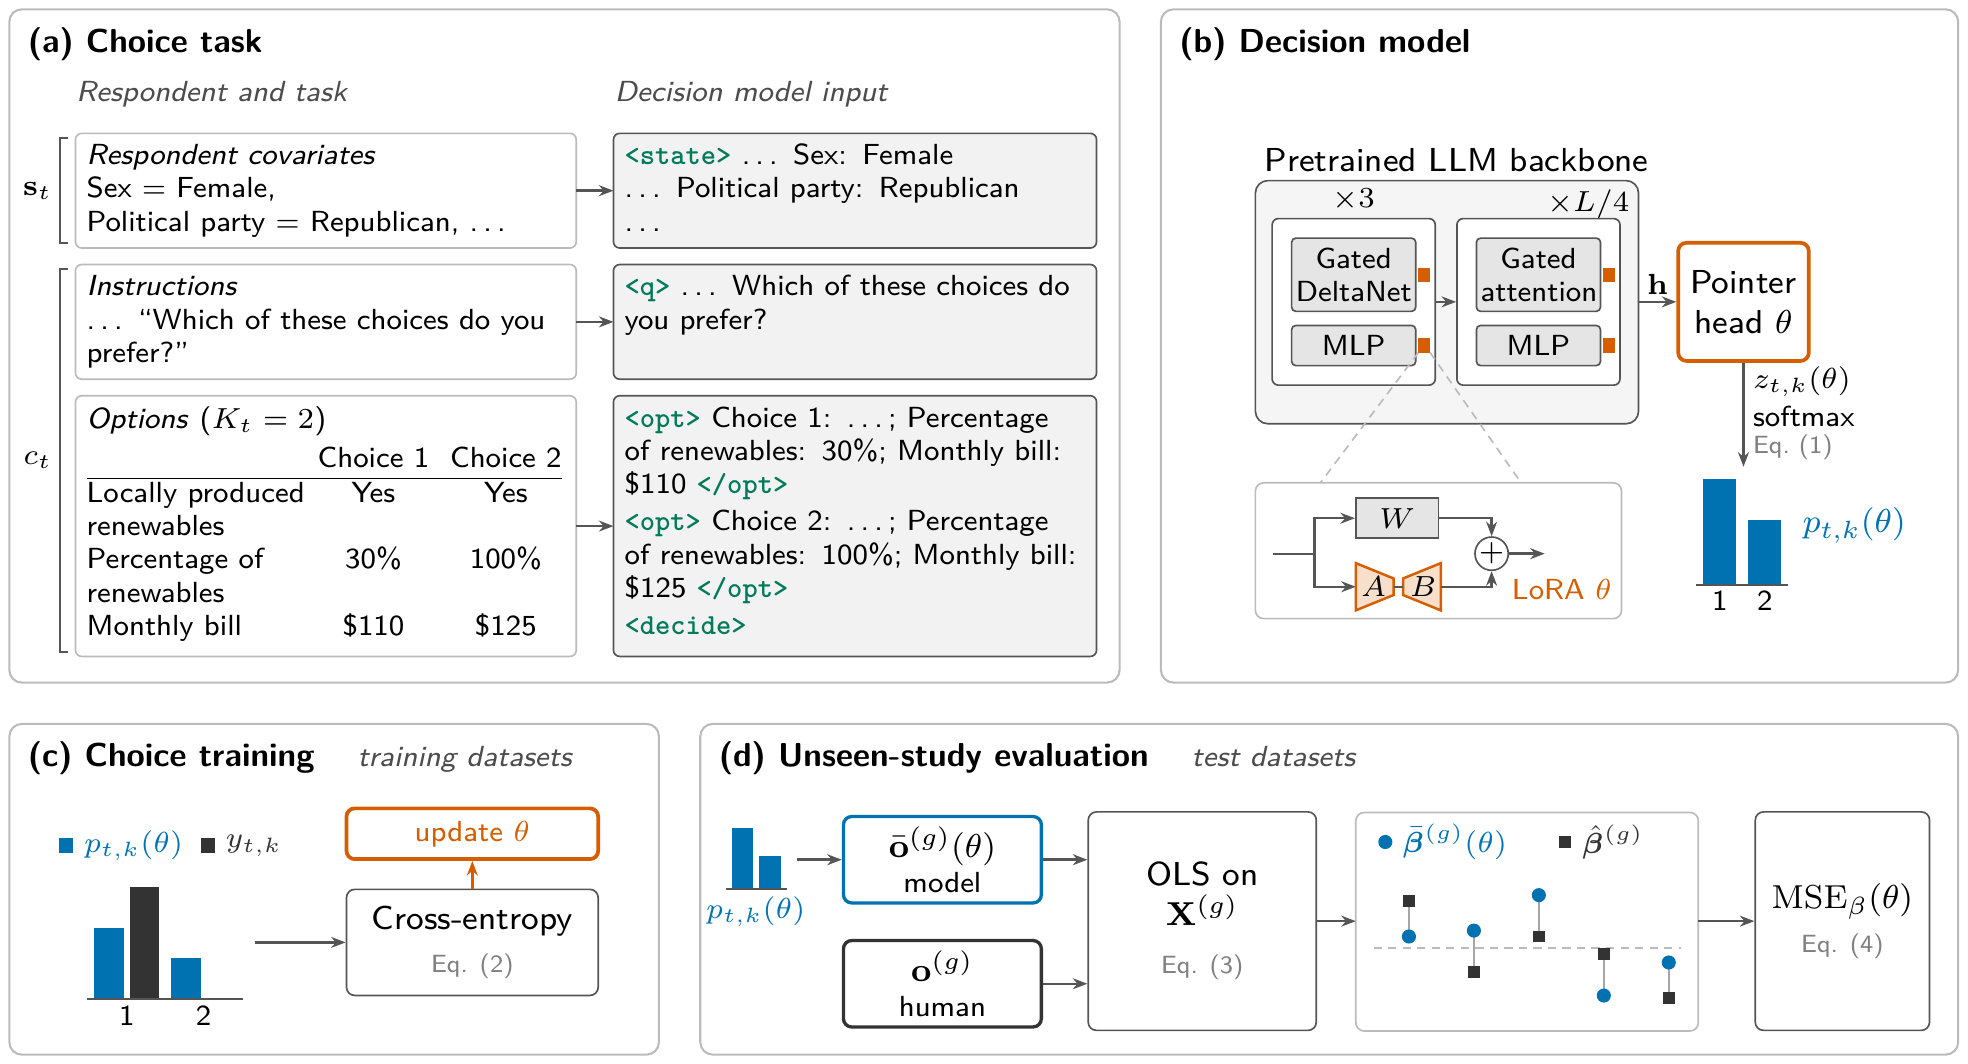
\includegraphics[width=1\linewidth,height=\textheight,keepaspectratio]{diagrams-tikz/fig_pipeline_v5.png}

}

\caption{\label{fig-pipeline}Choice training and unseen-study evaluation
of decision models}

\end{figure}%

\textbf{Decision model parameterization.} Consider a choice study
composed of discrete-choice tasks indexed by \(t\)
(Figure~\ref{fig-pipeline}, panel a). Each task pairs observed
respondent covariates \(\mathbf{s}_t\) (e.g., sex, age, education,
income, political affiliation, and race) with a task context \(c_t\)
specifying the instructions and \(K_t \ge 2\) discrete options. Let
\(y_{t,k} \in \{0, 1\}\) indicate whether the human respondent selects
option \(k \in \{1, \dots, K_t\}\) on task \(t\), with
\(\sum_{k=1}^{K_t} y_{t,k} = 1\).

Rather than generating text tokens autoregressively, a single-pass
decision model replaces the vocabulary head of a pretrained language
model with a pointer head that scores all \(K_t\) options in one forward
pass (Figure~\ref{fig-pipeline}, panel b). For each option \(k\), the
model computes a real-valued score \(z_{t,k}(\theta)\) from
\((\mathbf{s}_t, c_t)\), where \(\theta\) collects trainable low-rank
adaptation (LoRA) weights (Hu et al. 2021) on the backbone together with
the pointer-head parameters. Token serialization and query-key readout
equations appear in the Web Appendix. Applying a softmax transformation
with unit temperature produces the conditional choice probabilities:
\begin{equation}\protect\phantomsection\label{eq-model-pmf}{
p_{t,k}(\theta) = P\big(y_{t,k} = 1 \mid \mathbf{s}_t, c_t; \theta\big) = \frac{\exp\!\big(z_{t,k}(\theta)\big)}{\sum_{m=1}^{K_t} \exp\!\big(z_{t,m}(\theta)\big)}.
}\end{equation} Formally, Equation~\ref{eq-model-pmf} takes the
conditional multinomial logit form (McFadden 1972, Train 2009) with
\(z_{t,k}(\theta)\) acting as systematic utility. Because
Equation~\ref{eq-model-pmf} normalizes directly over
\(\{1, \dots, K_t\}\) without text decoding, refusals and out-of-set
outputs have zero probability by construction.

\textbf{Choice training.} Off-the-shelf decision models are pretrained
on objective single-label benchmarks where each task has a single
correct answer (Gao et al. 2026, Palmer 2026). Training on deterministic
labels widens score gaps across options and pushes predicted
probabilities \(p_{t,k}(\theta)\) toward zero and one. In human choice
studies, however, respondents with identical observed covariates
\(\mathbf{s}_t\) still differ in unobserved preferences. Therefore, the
true conditional choice distribution spreads probability mass across
options rather than collapsing onto a single mode.

Whereas post-inference adjustment and reweighting methods keep model
parameters fixed and require human data from the target study (Leng et
al. 2026, Wang et al. 2026), choice training updates \(\theta\) before
inference on historical respondent-level choice microdata
(Figure~\ref{fig-pipeline}, panel c). Starting from the off-the-shelf
model checkpoint, we treat repeated tasks per respondent marginally
under a pooled conditional log-likelihood and minimize empirical
cross-entropy over mini-batches \(S\) of historical tasks:
\begin{equation}\protect\phantomsection\label{eq-resp-ce}{
\mathcal{L}_{\mathrm{CE}}(\theta; S) = -\frac{1}{|S|} \sum_{t \in S} \sum_{k=1}^{K_t} y_{t,k} \log p_{t,k}(\theta).
}\end{equation} Minimizing Equation~\ref{eq-resp-ce} is equivalent to
pooled conditional maximum likelihood estimation of
Equation~\ref{eq-model-pmf}. Because cross-entropy is a strictly proper
scoring rule, its population minimizer recovers true conditional choice
probabilities rather than a deterministic mode. Importantly, no
target-study data enters Equation~\ref{eq-resp-ce}, so downstream
evaluation measures unseen-study transfer.

\textbf{Econometric evaluation.} On an unseen evaluation study, we hold
\(\theta\) fixed and evaluate treatment-effect recovery using ordinary
least squares (OLS) regressions defined by the study's experimental
design (Figure~\ref{fig-pipeline}, panel d). Applying the same linear
specification symmetrically to both human responses and model-implied
expected outcomes places the human benchmark and synthetic choice data
on a common estimator. Consider each regression
\(g \in \{1, \dots, G\}\) in the study, with full-column-rank design
matrix \(\mathbf{X}^{(g)}\) and human outcome vector
\(\mathbf{o}^{(g)}\). The matrix \(\mathbf{X}^{(g)}\) contains an
intercept and \(d_g\) treatment or attribute indicators from the
randomized design. Across all evaluation designs, each entry of
\(\mathbf{o}^{(g)}\) is a linear function of the choice indicators
\(y_{t,k}\). Specifically, it records a profile-selection indicator in
paired conjoints (zero across profiles when an opt-out is chosen), a
target-option indicator in binary-endpoint trials, or the numeric score
\(\sum_{k=1}^{K_t} k\,y_{t,k}\) in ordinal rating tasks. Replacing each
realized indicator \(y_{t,k}\) with its predicted probability
\(p_{t,k}(\theta)\) from Equation~\ref{eq-model-pmf} therefore yields
the exact expected outcome vector \(\bar{\mathbf{o}}^{(g)}(\theta)\)
under synthetic choice draws.

Applying the OLS operator
\(\mathbf{A}^{(g)} = (\mathbf{X}^{(g)\top}\mathbf{X}^{(g)})^{-1}\mathbf{X}^{(g)\top}\)
to the human and model-implied outcome vectors defines the intercepts
and slopes: \begin{equation}\protect\phantomsection\label{eq-pop-ols}{
\begin{pmatrix}
\hat{\alpha}^{(g)} \\
\hat{\boldsymbol{\beta}}^{(g)}
\end{pmatrix}
= \mathbf{A}^{(g)}\mathbf{o}^{(g)},
\qquad
\begin{pmatrix}
\bar{\alpha}^{(g)}(\theta) \\
\bar{\boldsymbol{\beta}}^{(g)}(\theta)
\end{pmatrix}
= \mathbf{A}^{(g)}\bar{\mathbf{o}}^{(g)}(\theta),
}\end{equation} where \(\hat{\alpha}^{(g)}\) and
\(\bar{\alpha}^{(g)}(\theta)\) are the intercepts,
\(\hat{\boldsymbol{\beta}}^{(g)}\) is the full-sample human slope
benchmark, and \(\bar{\boldsymbol{\beta}}^{(g)}(\theta)\) collects the
\(d_g\) model-implied treatment or attribute slopes. Because
\(\mathbf{X}^{(g)}\) is fixed and OLS is linear in the outcome vector,
\(\bar{\boldsymbol{\beta}}^{(g)}(\theta)\) equals the exact expectation
of the OLS slope estimator over synthetic choices drawn from
\(p_{t,k}(\theta)\), with zero Monte Carlo variance. Note that
Equation~\ref{eq-pop-ols} targets point-estimate recovery rather than
plug-in standard errors, because regressing deterministic expectations
\(\bar{\mathbf{o}}^{(g)}(\theta)\) omits realization-level sampling
variance.

Because all \(G\) regressions within each study share identical outcome
units, we measure aggregate slope recovery across all
\(d = \sum_{g=1}^G d_g\) slopes via mean squared error (Wang et al.
2026): \begin{equation}\protect\phantomsection\label{eq-eval-mse}{
\mathrm{MSE}_{\beta}(\theta) = \frac{1}{d} \sum_{g=1}^G \left\lVert \bar{\boldsymbol{\beta}}^{(g)}(\theta) - \hat{\boldsymbol{\beta}}^{(g)} \right\rVert_2^2.
}\end{equation} As a complementary individual-level diagnostic, we also
report held-out empirical cross-entropy in nats by evaluating
Equation~\ref{eq-resp-ce} over all tasks in each unseen study alongside
Equation~\ref{eq-eval-mse} in Table~\ref{tbl-results-mse}.

\section{Experimental setup}\label{sec-setup}

\subsection{Datasets and transfer
design}\label{datasets-and-transfer-design}

We evaluate choice training across seven choice datasets spanning
various product and policy domains, with no overlap between training,
validation, and testing (Table~\ref{tbl-datasets}). Two datasets provide
respondent-level training microdata: a paired electricity-plan conjoint
(\texttt{Electricity}; Wu 2025), and a discrete-choice experiment on
drone versus ground delivery across four vendor contexts
(\texttt{Drones}; Berke et al. 2023). Both training datasets vary price
(monthly bill or delivery fee) alongside non-price attributes. To
prevent held-out test datasets from informing model selection, we
designate the \texttt{Flights} dataset (Goldfarb et al. 2026) as a
dedicated validation dataset that selects every training run's
checkpoint.

Our four held-out test datasets never enter training, hyperparameter
tuning, or checkpoint selection. Two include price over wider ranges
than training (\texttt{Consumer\ rights} and
\texttt{AI\ \&\ offshoring}), whereas the other two share no attributes
with training (\texttt{Food\ labels} and \texttt{Vaccines}). Together,
these test datasets span paired conjoints, a three-option conjoint with
an opt-out (\texttt{Vaccines}), a five-point ordinal rating conjoint
(\texttt{AI\ \&\ offshoring}), and a six-arm randomized trial
(\texttt{Food\ labels}). Across all seven datasets, each choice task
conditions on the respondent's observed covariates \(\mathbf{s}_t\) in a
standardized text format (Figure~\ref{fig-pipeline}, panel a; mappings
appear in the Web Appendix).

\begin{longtable}[]{@{}
  >{\raggedright\arraybackslash}p{(\linewidth - 12\tabcolsep) * \real{0.1158}}
  >{\raggedright\arraybackslash}p{(\linewidth - 12\tabcolsep) * \real{0.1832}}
  >{\raggedright\arraybackslash}p{(\linewidth - 12\tabcolsep) * \real{0.2084}}
  >{\raggedright\arraybackslash}p{(\linewidth - 12\tabcolsep) * \real{0.2189}}
  >{\raggedleft\arraybackslash}p{(\linewidth - 12\tabcolsep) * \real{0.1368}}
  >{\raggedleft\arraybackslash}p{(\linewidth - 12\tabcolsep) * \real{0.0863}}
  >{\raggedleft\arraybackslash}p{(\linewidth - 12\tabcolsep) * \real{0.0505}}@{}}
\caption{Summary of training, validation, and held-out test
datasets}\label{tbl-datasets}\tabularnewline
\toprule\noalign{}
\begin{minipage}[b]{\linewidth}\raggedright
Role
\end{minipage} & \begin{minipage}[b]{\linewidth}\raggedright
Dataset
\end{minipage} & \begin{minipage}[b]{\linewidth}\raggedright
Price attributes
\end{minipage} & \begin{minipage}[b]{\linewidth}\raggedright
Non-price attributes
\end{minipage} & \begin{minipage}[b]{\linewidth}\raggedleft
Respondents
\end{minipage} & \begin{minipage}[b]{\linewidth}\raggedleft
Tasks
\end{minipage} & \begin{minipage}[b]{\linewidth}\raggedleft
\(d\)
\end{minipage} \\
\midrule\noalign{}
\endfirsthead
\toprule\noalign{}
\begin{minipage}[b]{\linewidth}\raggedright
Role
\end{minipage} & \begin{minipage}[b]{\linewidth}\raggedright
Dataset
\end{minipage} & \begin{minipage}[b]{\linewidth}\raggedright
Price attributes
\end{minipage} & \begin{minipage}[b]{\linewidth}\raggedright
Non-price attributes
\end{minipage} & \begin{minipage}[b]{\linewidth}\raggedleft
Respondents
\end{minipage} & \begin{minipage}[b]{\linewidth}\raggedleft
Tasks
\end{minipage} & \begin{minipage}[b]{\linewidth}\raggedleft
\(d\)
\end{minipage} \\
\midrule\noalign{}
\endhead
\bottomrule\noalign{}
\endlastfoot
Training & Electricity (Wu 2025) & Monthly bill (\$105 to \$125) &
Renewable share (10\% to 100\%), local renewables & 1,861 & 18,591 &
8 \\
Training & Drones (Berke et al. 2023) & Delivery fee (\$0 to \$10) &
Wait time, drone privacy & 3,625 & 36,297 & 28 \\
Validation & Flights (Goldfarb et al. 2026) & Ticket price (\$250 to
\$325) & Sustainable aviation fuel, airline, baggage, legroom, seat &
1,000 & 5,000 & 12 \\
Test & Consumer rights (Kantorowicz-Reznichenko et al. 2026) & Laptop
(\$500 to \$2,000) and laundry (\$400 to \$1,400) price & Brand, specs,
warranty, privacy, liability, conflict resolution & 2,242 & 26,823 &
38 \\
Test & AI \& offshoring (Magistro et al. 2026) & Smartphone price (\$300
to \$600) & Customer service, factory, and data science jobs & 5,525 &
21,005 & 32 \\
Test & Food labels (Grummon et al. 2025) & None & Front-of-package
warning labels (6 arms) & 5,633 & 33,798 & 5 \\
Test & Vaccines (Kreps et al. 2020) & None & Efficacy, duration, side
effects, FDA, origin, endorsements & 1,971 & 9,855 & 11 \\
\end{longtable}

\emph{Note.} Shorthand dataset labels in the Dataset column are used
throughout all tables and figures. The column \(d\) reports the total
number of non-reference treatment or attribute slopes across each
dataset's experimental design (Section~\ref{sec-methodology}).
Specifically, \texttt{Drones} spans four vendor contexts of 7 slopes
each (28 total), \texttt{Consumer\ rights} spans two product conjoints
of 19 slopes each (38 total), and \texttt{AI\ \&\ offshoring} spans four
country-by-arm regressions of 8 slopes each (32 total) on a five-point
support scale (1 to 5). Training datasets (\texttt{Electricity} and
\texttt{Drones}) enter exclusively as respondent-level choice microdata
via Equation~\ref{eq-resp-ce}, whereas validation and test datasets are
evaluated via Equation~\ref{eq-pop-ols} and Equation~\ref{eq-eval-mse}.

\subsection{Choice-training regimes}\label{choice-training-regimes}

Across every model scale, we evaluate a \(2 \times 2\) choice-training
design toggling inclusion of \texttt{Electricity} and \texttt{Drones}
across four regimes. \texttt{Off-the-shelf} evaluates the unmodified
decision model without choice training (\(0\) steps).
\texttt{Electricity} trains on the 18,591 choice tasks from Wu (2025)
(1,395 steps over \(3\) epochs), whereas \texttt{Drones} trains on the
36,297 choice tasks from Berke et al. (2023) (2,730 steps over \(3\)
epochs). Finally, \texttt{Drones\ +\ Electricity} pools all 54,888
choice tasks from both datasets under Equation~\ref{eq-resp-ce} (4,125
steps over \(3\) epochs). This factorial design isolates whether
single-dataset training already transfers to unseen datasets, whether
training-domain composition matters, and whether pooling distinct choice
datasets compounds unseen-study gains.

\subsection{Models, training protocol, and
evaluation}\label{models-training-protocol-and-evaluation}

We evaluate the \texttt{KEV-0.8B}, \texttt{KEV-4B}, and \texttt{KEV-9B}
open-weight decision models (Palmer 2026), each loaded in
\texttt{bfloat16} precision with unit temperature. Choice training
updates LoRA adapters (rank \(r = 64\), scaling
\(\alpha_{\mathrm{LoRA}} = 128\), dropout \(0.05\)) across all linear
backbone projections jointly with the trainable pointer head via
Equation~\ref{eq-resp-ce}. Every trained run uses AdamW with a
\(5 \times 10^{-6}\) peak learning rate, a OneCycle schedule (\(10\%\)
warmup and cosine decay), weight decay \(0.01\), and gradient-norm
clipping at \(1.0\). Training runs for \(3\) epochs with mini-batch size
\(|S| = 40\) and random seed \(42\). Within each epoch, tasks are
shuffled independently within each dataset (and within each vendor
context in \texttt{Drones}), partitioned into single-dataset
mini-batches, and interleaved randomly. We validate each run on
\texttt{Flights} at step \(0\), every \(32\) steps (\(1,280\) tasks),
and the final step, selecting the checkpoint with the lowest validation
\(\mathrm{MSE}_\beta\) (Equation~\ref{eq-eval-mse}). Main-text results
in Table~\ref{tbl-results-mse} report \(\mathrm{MSE}_\beta\)
(Equation~\ref{eq-eval-mse}) multiplied by \(10^3\) alongside held-out
empirical cross-entropy in nats (Equation~\ref{eq-resp-ce}). The Web
Appendix reports the off-the-shelf generative LLM protocol used in
Figure~\ref{fig-intro-off-the-shelf}
(\quartoapptblref{apptbl-llm-baseline}) and full attribute-level slope
tables and subset diagnostics (\quartoappfigref{appfig-flights-slopes};
\quartoapptblref{apptbl-vaccines-slopes} through
\quartoapptblref{apptbl-magistro-subsets}).

\section{Results}\label{sec-results}

\subsection{Unseen-study transfer across domains and model
scales}\label{unseen-study-transfer-across-domains-and-model-scales}

Table~\ref{tbl-results-mse} and Figure~\ref{fig-results-overall} report
unseen-study treatment-effect error (\(\mathrm{MSE}_\beta\)) and
held-out empirical cross-entropy (CE) across all three model scales,
four choice-training regimes, and five evaluation datasets. Pooled
choice training (\texttt{Drones\ +\ Electricity}) lowers
\(\mathrm{MSE}_\beta\) relative to the off-the-shelf checkpoint in all
15 model-dataset cells, including all 12 held-out test cells, and
achieves the lowest CE in every cell. Across held-out test datasets,
\(\mathrm{MSE}_\beta\) falls by 22\% to 89\%. These gains extend well
beyond \texttt{Flights} and the two held-out price datasets
(\texttt{Consumer\ rights} and \texttt{AI\ \&\ offshoring}). Some of the
sharpest improvements occur on non-price test datasets that share no
attributes with training, cutting \(\mathrm{MSE}_\beta\) by 79\% to 88\%
on \texttt{Vaccines} and by 35\% to 89\% on \texttt{Food\ labels} across
scales. Choice training also transfers across response formats, moving
from binary paired choices in training to three-option opt-out conjoints
(\texttt{Vaccines}), a six-arm randomized trial (\texttt{Food\ labels}),
and five-point ordinal ratings (\texttt{AI\ \&\ offshoring}). On
\texttt{AI\ \&\ offshoring}, larger raw \(\mathrm{MSE}_\beta\) values
reflect the 1 to 5 outcome scale rather than a binary indicator
(\quartoapptblref{apptbl-magistro-subsets}).

Comparing single-dataset regimes against \texttt{Drones\ +\ Electricity}
shows why pooling distinct choice datasets matters
(Table~\ref{tbl-results-mse} and Figure~\ref{fig-results-overall}).
Training on \texttt{Electricity} or \texttt{Drones} alone already
improves \(\mathrm{MSE}_\beta\) substantially on binary and three-option
tasks, yet both single-dataset regimes falter when moving from binary
choices to five-point ordinal ratings on \texttt{AI\ \&\ offshoring}.
Each single-dataset regime worsens \texttt{AI\ \&\ offshoring}
\(\mathrm{MSE}_\beta\) on two of the three model scales relative to the
off-the-shelf checkpoint. Pooling \texttt{Drones\ +\ Electricity}
reverses every one of those error increases, lowering
\texttt{AI\ \&\ offshoring} \(\mathrm{MSE}_\beta\) by 22\% to 35\%
across scales. Overall, pooled choice training attains the lowest
\(\mathrm{MSE}_\beta\) among all four regimes in 13 of 15 cells. It
trails a single-dataset model only on \texttt{KEV-9B} for
\texttt{Consumer\ rights} and \texttt{Food\ labels}, while still
recording the lowest CE in both cells.

Across model scales, choice training dominates off-the-shelf parameter
scaling. Echoing the off-the-shelf generative LLM pattern in
Figure~\ref{fig-intro-off-the-shelf}, scaling off-the-shelf decision
models from \texttt{KEV-0.8B} to \texttt{KEV-9B} does not reliably
improve treatment-effect recovery. Off-the-shelf \texttt{KEV-9B} incurs
higher \(\mathrm{MSE}_\beta\) than off-the-shelf \texttt{KEV-0.8B} on
three of the four held-out test datasets (\texttt{AI\ \&\ offshoring},
\texttt{Food\ labels}, and \texttt{Vaccines}), improving monotonically
with scale only on \texttt{Consumer\ rights}. By contrast, pooled choice
training overturns an order-of-magnitude gap in parameter count.
Choice-trained \texttt{KEV-0.8B} outperforms off-the-shelf
\texttt{KEV-9B} on four of five datasets, trailing only on
\texttt{Consumer\ rights}. At the middle scale, choice-trained
\texttt{KEV-4B} achieves the lowest \(\mathrm{MSE}_\beta\) overall on
\texttt{Flights}, \texttt{Food\ labels}, and \texttt{Vaccines}, and
virtually matches choice-trained \texttt{KEV-9B} on
\texttt{AI\ \&\ offshoring}.

The CE columns in Table~\ref{tbl-results-mse} clarify why off-the-shelf
scaling breaks down and confirm that aggregate OLS slope gains reflect
genuine individual-level probability improvements. Consistent with the
objective-pretraining mechanism in Section~\ref{sec-methodology},
off-the-shelf decision models exhibit severe overconfidence. Their
held-out CE (Equation~\ref{eq-resp-ce}) exceeds uniform random guessing
(\(\ln K\), with \(K \in \{2, 3, 5\}\) in Table~\ref{tbl-datasets}) in
14 of 15 cells. Moreover, off-the-shelf CE rises with parameter scale on
\texttt{Food\ labels}, \texttt{Vaccines}, and
\texttt{AI\ \&\ offshoring}. Larger off-the-shelf models thus
concentrate probability mass even more sharply onto extreme options,
amplifying OLS slope distortion. Pooled choice training reverses this
collapse across every scale and dataset. It lowers CE strictly below
\(\ln K\) in 11 of 15 cells and brings the remaining cells close to or
effectively at that threshold, cutting CE by roughly 0.7 to 0.8 nats
across scales on five-point \texttt{AI\ \&\ offshoring}. Because
Equation~\ref{eq-resp-ce} penalizes misallocated respondent-level
probabilities directly, these parallel drops in CE and
\(\mathrm{MSE}_\beta\) (Equation~\ref{eq-eval-mse}) rule out slope-level
error cancellation across respondents or attributes.

\nexttablesize{\scriptsize}

\begin{longtable}[]{@{}
  >{\raggedright\arraybackslash}p{(\linewidth - 20\tabcolsep) * \real{0.1547}}
  >{\raggedleft\arraybackslash}p{(\linewidth - 20\tabcolsep) * \real{0.0868}}
  >{\raggedleft\arraybackslash}p{(\linewidth - 20\tabcolsep) * \real{0.0755}}
  >{\raggedleft\arraybackslash}p{(\linewidth - 20\tabcolsep) * \real{0.0868}}
  >{\raggedleft\arraybackslash}p{(\linewidth - 20\tabcolsep) * \real{0.0755}}
  >{\raggedleft\arraybackslash}p{(\linewidth - 20\tabcolsep) * \real{0.0868}}
  >{\raggedleft\arraybackslash}p{(\linewidth - 20\tabcolsep) * \real{0.0755}}
  >{\raggedleft\arraybackslash}p{(\linewidth - 20\tabcolsep) * \real{0.0868}}
  >{\raggedleft\arraybackslash}p{(\linewidth - 20\tabcolsep) * \real{0.0755}}
  >{\raggedleft\arraybackslash}p{(\linewidth - 20\tabcolsep) * \real{0.0868}}
  >{\raggedleft\arraybackslash}p{(\linewidth - 20\tabcolsep) * \real{0.0755}}@{}}

\caption{\label{tbl-results-mse}OLS treatment-effect error and empirical
cross-entropy across datasets and choice-training regimes}

\tabularnewline

\toprule\noalign{}
\multirow{2}{=}{\begin{minipage}[b]{\linewidth}\raggedright
Trained on
\end{minipage}} &
\multicolumn{2}{>{\centering\arraybackslash}p{(\linewidth - 20\tabcolsep) * \real{0.1623} + 2\tabcolsep}}{%
\begin{minipage}[b]{\linewidth}\centering
Flights
\end{minipage}} &
\multicolumn{2}{>{\centering\arraybackslash}p{(\linewidth - 20\tabcolsep) * \real{0.1623} + 2\tabcolsep}}{%
\begin{minipage}[b]{\linewidth}\centering
Consumer rights
\end{minipage}} &
\multicolumn{2}{>{\centering\arraybackslash}p{(\linewidth - 20\tabcolsep) * \real{0.1623} + 2\tabcolsep}}{%
\begin{minipage}[b]{\linewidth}\centering
AI \& offshoring
\end{minipage}} &
\multicolumn{2}{>{\centering\arraybackslash}p{(\linewidth - 20\tabcolsep) * \real{0.1623} + 2\tabcolsep}}{%
\begin{minipage}[b]{\linewidth}\centering
Food labels
\end{minipage}} &
\multicolumn{2}{>{\centering\arraybackslash}p{(\linewidth - 20\tabcolsep) * \real{0.1623} + 2\tabcolsep}@{}}{%
\begin{minipage}[b]{\linewidth}\centering
Vaccines
\end{minipage}} \\
& \begin{minipage}[b]{\linewidth}\raggedleft
\(\mathrm{MSE}_\beta\)
\end{minipage} & \begin{minipage}[b]{\linewidth}\raggedleft
CE
\end{minipage} & \begin{minipage}[b]{\linewidth}\raggedleft
\(\mathrm{MSE}_\beta\)
\end{minipage} & \begin{minipage}[b]{\linewidth}\raggedleft
CE
\end{minipage} & \begin{minipage}[b]{\linewidth}\raggedleft
\(\mathrm{MSE}_\beta\)
\end{minipage} & \begin{minipage}[b]{\linewidth}\raggedleft
CE
\end{minipage} & \begin{minipage}[b]{\linewidth}\raggedleft
\(\mathrm{MSE}_\beta\)
\end{minipage} & \begin{minipage}[b]{\linewidth}\raggedleft
CE
\end{minipage} & \begin{minipage}[b]{\linewidth}\raggedleft
\(\mathrm{MSE}_\beta\)
\end{minipage} & \begin{minipage}[b]{\linewidth}\raggedleft
CE
\end{minipage} \\
\midrule\noalign{}
\endhead
\bottomrule\noalign{}
\endlastfoot
\multicolumn{11}{@{}>{\centering\arraybackslash}p{(\linewidth - 20\tabcolsep) * \real{0.9660} + 20\tabcolsep}@{}}{%
\emph{KEV-0.8B}} \\
Off-the-shelf & 17.75 & 1.086 & 8.34 & 1.418 & 33.92 & 2.283 & 5.46 &
1.059 & 12.07 & 1.185 \\
Electricity & 8.91 & 0.693 & 7.35 & 0.821 & 29.60 & 1.689 & 3.53 & 0.915
& 3.73 & 1.082 \\
Drones & 9.68 & 0.709 & 7.17 & 0.806 & 34.41 & 1.630 & 3.25 & 0.953 &
4.08 & 1.105 \\
Drones + Electricity & \textbf{4.62} & \textbf{0.647} & \textbf{6.04} &
\textbf{0.695} & \textbf{26.61} & \textbf{1.558} & \textbf{2.30} &
\textbf{0.879} & \textbf{2.56} & \textbf{1.067} \\
\multicolumn{11}{@{}>{\centering\arraybackslash}p{(\linewidth - 20\tabcolsep) * \real{0.9660} + 20\tabcolsep}@{}}{%
\emph{KEV-4B}} \\
Off-the-shelf & 4.10 & 0.811 & 4.89 & 0.779 & 99.01 & 2.434 & 21.10 &
1.100 & 9.08 & 1.525 \\
Electricity & 1.72 & 0.625 & 3.27 & 0.650 & 113.26 & 1.886 & 3.57 &
0.887 & 1.73 & 1.120 \\
Drones & 1.00 & 0.623 & 2.64 & 0.663 & 74.69 & 1.797 & 7.04 & 0.959 &
4.63 & 1.195 \\
Drones + Electricity & \textbf{0.73} & \textbf{0.588} & \textbf{2.25} &
\textbf{0.629} & \textbf{63.98} & \textbf{1.636} & \textbf{2.28} &
\textbf{0.854} & \textbf{1.12} & \textbf{1.046} \\
\multicolumn{11}{@{}>{\centering\arraybackslash}p{(\linewidth - 20\tabcolsep) * \real{0.9660} + 20\tabcolsep}@{}}{%
\emph{KEV-9B}} \\
Off-the-shelf & 5.12 & 0.833 & 1.76 & 0.804 & 82.89 & 2.437 & 22.73 &
1.238 & 14.30 & 1.422 \\
Electricity & 2.17 & 0.647 & \textbf{1.34} & 0.694 & 95.68 & 1.873 &
18.85 & 0.972 & 4.25 & 1.203 \\
Drones & 2.62 & 0.646 & 1.37 & 0.674 & 87.42 & 2.000 & \textbf{10.90} &
0.963 & 9.54 & 1.165 \\
Drones + Electricity & \textbf{0.93} & \textbf{0.604} & 1.36 &
\textbf{0.665} & \textbf{63.49} & \textbf{1.658} & 14.82 &
\textbf{0.808} & \textbf{2.43} & \textbf{1.100} \\

\end{longtable}

\emph{Note.} \(\mathrm{MSE}_\beta\) reports population OLS
treatment-effect error \(\times 10^3\) (Equation~\ref{eq-eval-mse}) and
CE reports mean empirical cross-entropy (negative log-likelihood per
choice task, in nats; Equation~\ref{eq-resp-ce}); lower is better for
both metrics. Uniform random guessing yields
\(\mathrm{CE} = \ln 2 = 0.693\) on \texttt{Flights} and
\texttt{Consumer\ rights}, \(\ln 3 = 1.099\) on \texttt{Food\ labels}
and \texttt{Vaccines}, and \(\ln 5 = 1.609\) on
\texttt{AI\ \&\ offshoring}. Bold marks the lowest value per model,
dataset, and metric. \texttt{Flights} is the validation dataset that
selects each run's checkpoint; \texttt{Consumer\ rights} and
\texttt{AI\ \&\ offshoring} are held-out test price datasets;
\texttt{Food\ labels} and \texttt{Vaccines} are held-out test non-price
datasets.

\begin{figure}

\centering{

\includegraphics[width=1\linewidth,height=\textheight,keepaspectratio]{manuscript-training-assets/fig-results-overall.png}

}

\caption{\label{fig-results-overall}Population OLS treatment-effect
error across datasets and choice-training regimes}

\end{figure}%

\subsection{Attribute-level transfer across shared and unseen
attributes}\label{attribute-level-transfer-across-shared-and-unseen-attributes}

Because both training datasets include a price attribute, aggregate
\(\mathrm{MSE}_\beta\) reductions could in principle stem from price
sensitivity transferring alone while unseen non-price attributes remain
distorted. Attribute-level estimates on held-out
\texttt{Consumer\ rights} rule out that explanation
(Figure~\ref{fig-results-laptops-slopes}; full laptop and laundry
estimates in \quartoapptblref{apptbl-consumer-rights-slopes}). Across
all 34 unseen non-price slopes, pooled choice training lowers non-price
\(\mathrm{MSE}_\beta\) at every model scale, by 24\% to 41\%. On
\texttt{KEV-9B}, where pooled training slightly overshoots price slopes
relative to the off-the-shelf model, the entire net improvement on
\texttt{Consumer\ rights} comes from unseen non-price attributes. In the
laptop conjoint (Figure~\ref{fig-results-laptops-slopes}), off-the-shelf
\texttt{KEV-0.8B} and \texttt{KEV-4B} compress hardware, warranty, and
price slopes toward zero while inverting brand and consumer-rights
signs. Pooled choice training lifts price, RAM, storage, and ten-year
warranty slopes toward the human benchmark and corrects inverted signs
on Apple MacBook, full privacy, and conflict resolution. Even so, brand
premia and ten-year warranty effects remain attenuated relative to human
choices.

The non-price \texttt{Vaccines} conjoint provides an even cleaner test
because it shares no attributes with either training dataset
(Figure~\ref{fig-results-vaccines-slopes} and
\quartoapptblref{apptbl-vaccines-slopes}). Here, choice training
corrects two opposite off-the-shelf distortions at once. First,
off-the-shelf models sharply exaggerate socially and politically salient
cues, overstating CDC and WHO endorsements across all three scales. At
\texttt{KEV-4B} and \texttt{KEV-9B}, they also overshoot high vaccine
efficacy and China-origin penalties. Pooled choice training cuts those
endorsement overshoots by more than half across scales and pulls
efficacy and origin slopes back toward human estimates. Second, choice
training simultaneously lifts underweighted clinical and regulatory
slopes rather than shrinking all effects toward zero. Across scales, it
raises five-year duration and severe side-effect slopes toward human
magnitudes and moderates the \texttt{KEV-4B} emergency-authorization
distortion. Because choice training pulls exaggerated slopes downward
while lifting suppressed slopes upward within the same task,
unseen-study transfer cannot be explained by simple temperature
rescaling or uniform shrinkage.

The remaining Web Appendix breakdowns reinforce both the breadth and the
limits of attribute-level transfer. On held-out \texttt{Food\ labels}
(\quartoapptblref{apptbl-food-slopes}), off-the-shelf \texttt{KEV-4B}
and \texttt{KEV-9B} invert the \texttt{HighIn} warning label into a
large negative slope while exaggerating nutrition-information arms.
Pooled choice training nearly eliminates that sign inversion and brings
\texttt{KEV-4B} close to human estimates across arms. On held-out
\texttt{AI\ \&\ offshoring}
(\quartoapptblref{apptbl-ai-offshoring-slopes} and
\quartoapptblref{apptbl-magistro-subsets}), pooled training cuts
non-price job-change \(\mathrm{MSE}_\beta\) by 33\% to 34\% across all
three scales and moderates extreme off-the-shelf overreactions to
factory-job gains. However, factory-job slopes remain inflated at
\texttt{KEV-4B} and \texttt{KEV-9B}, and \texttt{KEV-9B} overshoots
price slopes under the five-point ordinal scale. These residual gaps
underscore that transfer across response formats remains harder than
transfer within binary or three-option designs. Finally, the
\texttt{Flights} validation breakdown
(\quartoappfigref{appfig-flights-slopes} and
\quartoapptblref{apptbl-flights-slopes}) exhibits the same dual
improvement across shared price levels and unseen airline, baggage, and
sustainable-fuel attributes.

\begin{figure}

\centering{

\includegraphics[width=1\linewidth,height=\textheight,keepaspectratio]{manuscript-training-assets/fig-results-laptops-slopes.png}

}

\caption{\label{fig-results-laptops-slopes}Consumer rights (laptops) OLS
treatment effects by attribute for off-the-shelf and pooled
choice-trained models}

\end{figure}%

\begin{figure}

\centering{

\includegraphics[width=1\linewidth,height=\textheight,keepaspectratio]{manuscript-training-assets/fig-results-vaccines-slopes.png}

}

\caption{\label{fig-results-vaccines-slopes}Vaccines OLS treatment
effects by attribute for off-the-shelf and pooled choice-trained models}

\end{figure}%

\section{Conclusion}\label{sec-conclusion}

Off-the-shelf foundation models, whether autoregressive generative LLMs
or single-pass decision models, struggle to recover human treatment
effects in unseen choice studies. Contrary to common intuition, scaling
parameter count or increasing reasoning effort often intensifies
overconfidence and worsens downstream econometric error. We show that
pre-inference choice training on compact open-weight decision models
reverses this pattern. Training decision models with respondent-level
cross-entropy on just two historical choice datasets lowers unseen-study
OLS treatment-effect error and held-out cross-entropy across every model
scale. The improvement transfers across unseen domains, non-price
attributes, and new response formats without any target-study human
data.

These results carry two practical implications for marketing researchers
using synthetic respondents. First, pre-inference choice training
complements rather than replaces confirmatory human data collection and
post-inference adjustment (Hullman et al. 2026, Leng et al. 2026, Wang
et al. 2026). Improving how accurately the model captures human choice
uncertainty before inference strengthens exploratory pre-testing and
experimental design. It also shrinks the bias that post-inference
debiasing must correct once human validation data is collected. Second,
data diversity and architectural fit matter more than raw parameter
scale. Pooling distinct choice datasets avoids the higher errors that
single-dataset training suffers when transferring from binary choices to
five-point ordinal ratings. Moreover, a choice-trained mid-sized model
(\texttt{KEV-4B}) matches or outperforms a much larger model
(\texttt{KEV-9B}). Because it is a single-pass decision model, it
delivers exact choice probabilities with zero refusals and no Monte
Carlo sampling cost.

At the same time, our findings reveal an important limitation of
training solely on respondent-level cross-entropy. Although
cross-entropy is a strictly proper scoring rule for individual choice
probabilities, lower task-level cross-entropy does not automatically
guarantee lower downstream treatment-effect error. The held-out
\texttt{Food\ labels} results in Table~\ref{tbl-results-mse} illustrate
this tension clearly. There, pooled \texttt{KEV-9B} achieves the lowest
cross-entropy of any model and training regime, yet incurs the highest
\(\mathrm{MSE}_\beta\) among the pooled models. Its slope error exceeds
that of pooled \texttt{KEV-4B} by more than sixfold and even trails
\texttt{KEV-9B} trained on \texttt{Drones} alone. Because cross-entropy
weights every task-level log-probability equally without directly
penalizing bias in treatment-versus-control contrasts, probability gains
at the individual level can coexist with distorted experimental slopes.
Fortunately, single-pass decision models yield exact, differentiable
expected OLS slopes (Equation~\ref{eq-pop-ols}), creating a natural
avenue for future research that trains jointly on respondent-level
cross-entropy and a direct treatment-effect loss.

Several additional boundaries suggest further directions for research.
Even after pooled choice training, models still attenuate certain brand
and long-horizon warranty effects on \texttt{Consumer\ rights}.
Likewise, transfer to five-point ordinal ratings on
\texttt{AI\ \&\ offshoring} remains noticeably harder than transfer
across binary and three-option choice tasks. Moreover, our evaluation
targets population point-estimate recovery rather than plug-in standard
errors or subgroup-level heterogeneous treatment effects. Expanding
choice training beyond two binary US datasets to include ordinal scales,
opt-out tasks, non-US samples, and richer respondent covariates offers a
clear path toward more general, econometrically reliable synthetic
respondents.

\section*{Declarations}\label{declarations}
\addcontentsline{toc}{section}{Declarations}

\subsection*{Funding and competing
interests}\label{funding-and-competing-interests}
\addcontentsline{toc}{subsection}{Funding and competing interests}

All authors certify that they have no affiliations with or involvement
in any organization or entity with any financial interest or
non-financial interest in the subject matter or materials discussed in
this manuscript. The authors have no funding to report.

\section*{References}\label{references}
\addcontentsline{toc}{section}{References}

\protect\phantomsection\label{refs}
\begin{CSLReferences}{1}{0}
\bibitem[\citeproctext]{ref-argyle2023out}
Argyle LP, Busby EC, Fulda N, Gubler JR, Rytting C, Wingate D (2023) Out
of one, many: Using language models to simulate human samples.
\emph{Political Analysis} 31(3):337--351.

\bibitem[\citeproctext]{ref-arora2025ai}
Arora N, Chakraborty I, Nishimura Y (2025) AI--human hybrids for
marketing research: Leveraging large language models (LLMs) as
collaborators. \emph{Journal of Marketing} 89(2):43--70.

\bibitem[\citeproctext]{ref-berke2023drone}
Berke A, Ding G, Chin C, Gopalakrishnan K, Larson K, Balakrishnan H, Li
MZ (2023) Drone delivery and the value of customer privacy: A discrete
choice experiment with US consumers. \emph{Transportation Research Part
C: Emerging Technologies} 157:104391.

\bibitem[\citeproctext]{ref-binz2025foundation}
{Binz M, Akata E, Bethge M, Brändle F, Callaway F, Coda-Forno J, Dayan
P, et al.} (2025) A foundation model to predict and capture human
cognition. \emph{Nature} 644(8078):1002--1009.

\bibitem[\citeproctext]{ref-brand2023using}
Brand J, Israeli A, Ngwe D (2023) \emph{Using {LLMs} for market
research}. Working Paper 23-062 (Harvard Business School).

\bibitem[\citeproctext]{ref-deusser2026evaluatingbenchmarkingmodeljev}
Deußer T, Sparrenberg L, Sifa R (2026)
\href{https://arxiv.org/abs/2609.37647}{Evaluating and benchmarking the
system one model {Jev}}. \emph{arXiv preprint arXiv:2609.37647}.

\bibitem[\citeproctext]{ref-gao2026choicesfewerdecisionsordinalscale}
Gao T, Li J, Li Z, Chang Y, Wu Y (2026)
\href{https://arxiv.org/abs/2609.38827}{More choices, fewer decisions:
Ordinal-scale bias in {JEV}-like direct-decision models}. \emph{arXiv
preprint arXiv:2609.38827}.

\bibitem[\citeproctext]{ref-geuter2026releasinginnerjevsimple}
Geuter J, Cheng A, Alvarez-Melis D (2026)
\href{https://arxiv.org/abs/2610.17205}{Releasing the inner {Jev}: A
simple recipe for open decision models}. \emph{arXiv preprint
arXiv:2610.17205}.

\bibitem[\citeproctext]{ref-goldfarb2026comfort}
Goldfarb JL, Bhujle TR, Tester JW, Kriner DL (2026) Comfort or climate?
Consumer trade-offs between sustainable aviation fuel and flight
amenities. \emph{Journal of Cleaner Production} 577:149406.

\bibitem[\citeproctext]{ref-goli2024frontiers}
Goli A, Singh A (2024) Frontiers: Can large language models capture
human preferences? \emph{Marketing Science} 43(4):709--722.

\bibitem[\citeproctext]{ref-grummon2025nutrition}
Grummon AH, O'Sullivan K, Petimar J, Lee CJY, Zeitlin AB, Cleveland LP,
Collis C, et al. (2025) Nutrition info and other front-of-package labels
and simulated food and beverage purchases: A randomized clinical trial.
\emph{JAMA Network Open} 8(10):e2537389.
\url{https://doi.org/10.1001/jamanetworkopen.2025.37389}.

\bibitem[\citeproctext]{ref-horton2023large}
Horton JJ, Filippas A, Manning BS (2023) \emph{Large language models as
simulated economic agents: What can we learn from {Homo Silicus}?}
Working Paper 31122 (National Bureau of Economic Research).

\bibitem[\citeproctext]{ref-hu2021lora}
Hu EJ, Shen Y, Wallis P, Allen-Zhu Z, Li Y, Wang S, Wang L, Chen W
(2021) Lora: Low-rank adaptation of large language models. \emph{arXiv
preprint arXiv:2106.09685}.

\bibitem[\citeproctext]{ref-huang-etal-2026-distribution}
Huang J, Li M, Shao S (2026)
\href{https://doi.org/10.18653/v1/2026.findings-acl.457}{Distribution
shift alignment helps {LLM}s simulate survey response distributions}.
\emph{Findings of the {A}ssociation for {C}omputational {L}inguistics:
{ACL} 2026}, 9395--9409.

\bibitem[\citeproctext]{ref-hullman2026human}
Hullman J, Broska D, Sun H, Shaw A (2026) This human study did not
involve human subjects: Validating LLM simulations as behavioral
evidence. \emph{arXiv preprint arXiv:2602.15785}.

\bibitem[\citeproctext]{ref-kadavath2022language}
{Kadavath S, Conerly T, Askell A, Henighan T, Drain D, Perez E, Schiefer
N, et al.} (2022) Language models (mostly) know what they know.
\emph{arXiv preprint arXiv:2207.05221}.

\bibitem[\citeproctext]{ref-kantorowicz2026consumers}
Kantorowicz-Reznichenko E, Van Heusden A, Kantorowicz J (2026)
Consumers' rights in the shadow of the brand: A conjoint experiment on
the valuation and trade-offs of contractual rights. \emph{Journal of Law
\& Empirical Analysis} 3(1):105--126.

\bibitem[\citeproctext]{ref-kolluri2025finetuning}
Kolluri A, Wu S, Park JS, Bernstein MS (2025) Finetuning llms for human
behavior prediction in social science experiments. \emph{Proceedings of
the 2025 conference on empirical methods in natural language
processing}, 30084--30099.

\bibitem[\citeproctext]{ref-kreps2020factors}
Kreps S, Prasad S, Brownstein JS, Hswen Y, Garibaldi BT, Zhang B, Kriner
DL (2020) Factors associated with {US} adults' likelihood of accepting
COVID-19 vaccination. \emph{JAMA Network Open} 3(10):e2025594.

\bibitem[\citeproctext]{ref-ku2026siliconsamplingcrosssurveytransfer}
Ku CT, Hsu C, Huang PC, Liu FC, Cheng IL, Kang Y (2026)
\href{https://arxiv.org/abs/2607.03091}{Silicon sampling via
cross-survey transfer}. \emph{arXiv preprint arXiv:2607.03091}.

\bibitem[\citeproctext]{ref-leng2026reducing}
Leng Y, Sang Y, Agarwal A (2026) Reducing disparity between {LLM}s and
humans: Optimal {LLM} sample calibration. \emph{Marketing Science}.
\url{https://doi.org/10.1287/mksc.2024.0983}.

\bibitem[\citeproctext]{ref-magistro2026attitudes}
Magistro B, Borwein S, Alvarez RM, Bonikowski B, Loewen PJ (2026)
Attitudes toward artificial intelligence (AI) and globalization: Common
microfoundations and political implications. \emph{American Journal of
Political Science} 70(1):348--365.

\bibitem[\citeproctext]{ref-mcfadden1972conditional}
McFadden D (1972) Conditional logit analysis of qualitative choice
behavior.

\bibitem[\citeproctext]{ref-palmer2026kev}
Palmer J (2026) Kev: Small {Jev}-like decision models.
\url{https://github.com/jaredpalmer/kev}.

\bibitem[\citeproctext]{ref-pmlr-v202-santurkar23a}
Santurkar S, Durmus E, Ladhak F, Lee C, Liang P, Hashimoto T (2023)
\href{https://proceedings.mlr.press/v202/santurkar23a.html}{Whose
opinions do language models reflect?} \emph{Proceedings of the 40th
{International Conference on Machine Learning}}, 29971--30004.

\bibitem[\citeproctext]{ref-suh-etal-2025-language}
Suh J, Jahanparast E, Moon S, Kang M, Chang S (2025)
\href{https://doi.org/10.18653/v1/2025.acl-long.1028}{Language model
fine-tuning on scaled survey data for predicting distributions of public
opinions}. \emph{Proceedings of the 63rd annual meeting of the
{A}ssociation for {C}omputational {L}inguistics (volume 1: Long
papers)}, 21147--21170.

\bibitem[\citeproctext]{ref-toubia2025database}
Toubia O, Gui GZ, Peng T, Merlau DJ, Li A, Chen H (2025) Database
report: {Twin-2K-500}: A data set for building digital twins of over
2,000 people based on their answers to over 500 questions.
\emph{Marketing Science} 44(6):1446--1455.

\bibitem[\citeproctext]{ref-train2009discrete}
Train KE (2009) \emph{Discrete choice methods with simulation}
(Cambridge university press).

\bibitem[\citeproctext]{ref-wadi2025monte}
Wadi D, Fredette M (2025) A {Monte-Carlo} sampling framework for
reliable evaluation of large language models using behavioral analysis.
\emph{Findings of the {Association for Computational Linguistics}:
{EMNLP} 2025}, 9414--9432.

\bibitem[\citeproctext]{ref-wadi2026every}
Wadi D, Ghodrat M, Philp M (2026) Every token counts: Exact
{Likert}-scale distributions for measuring LLM attitudes and biases.
\emph{arXiv preprint arXiv:2608.10503}.

\bibitem[\citeproctext]{ref-wang2026large}
Wang M, Zhang DJ, Zhang H (2026) Large language models for market
research: A data-augmentation approach. \emph{Marketing Science}
45(4):728--751. \url{https://doi.org/10.1287/mksc.2025.0009}.

\bibitem[\citeproctext]{ref-wang2025can}
Wang S, Hunt K, Tang S, Joseph K (2025) Can finetuing LLMs on small
human samples increase heterogeneity, alignment, and belief-action
coherence? \emph{arXiv preprint arXiv:2511.21218}.

\bibitem[\citeproctext]{ref-wu2025partisan}
Wu VY (2025) Partisan energy preferences in the united states:
Republicans prioritize price, democrats also consider renewables.
\emph{Energy Research \& Social Science} 123:103997.

\bibitem[\citeproctext]{ref-ye2025fine}
Ye Z, Zhao J, Wang L (2025) Fine-tune, then rectify. \emph{arXiv
e-prints}:arXiv--2511.

\end{CSLReferences}

\newpage{}

\section*{Web Appendix}\label{web-appendix}
\addcontentsline{toc}{section}{Web Appendix}

\subsection*{Token serialization, query-key readout, and covariate
mappings}\label{token-serialization-query-key-readout-and-covariate-mappings}
\addcontentsline{toc}{subsection}{Token serialization, query-key
readout, and covariate mappings}

\begin{tcolorbox}[enhanced jigsaw, arc=.35mm, bottomrule=.15mm, bottomtitle=1mm, breakable, colback=white, colbacktitle=quarto-callout-note-color!10!white, colframe=quarto-callout-note-color-frame, coltitle=black, left=2mm, leftrule=.75mm, opacityback=0, opacitybacktitle=0.6, rightrule=.15mm, title=\textcolor{quarto-callout-note-color}{\faInfo}\hspace{0.5em}{Note}, titlerule=0mm, toprule=.15mm, toptitle=1mm]

\textbf{TODO.} Add token serialization equations, query-key readout
equations, and respondent-covariate mapping tables across all seven
datasets alongside \quartoappfigref{appfig-input-vaccines}.

\end{tcolorbox}

\begin{appfig}

\centering{

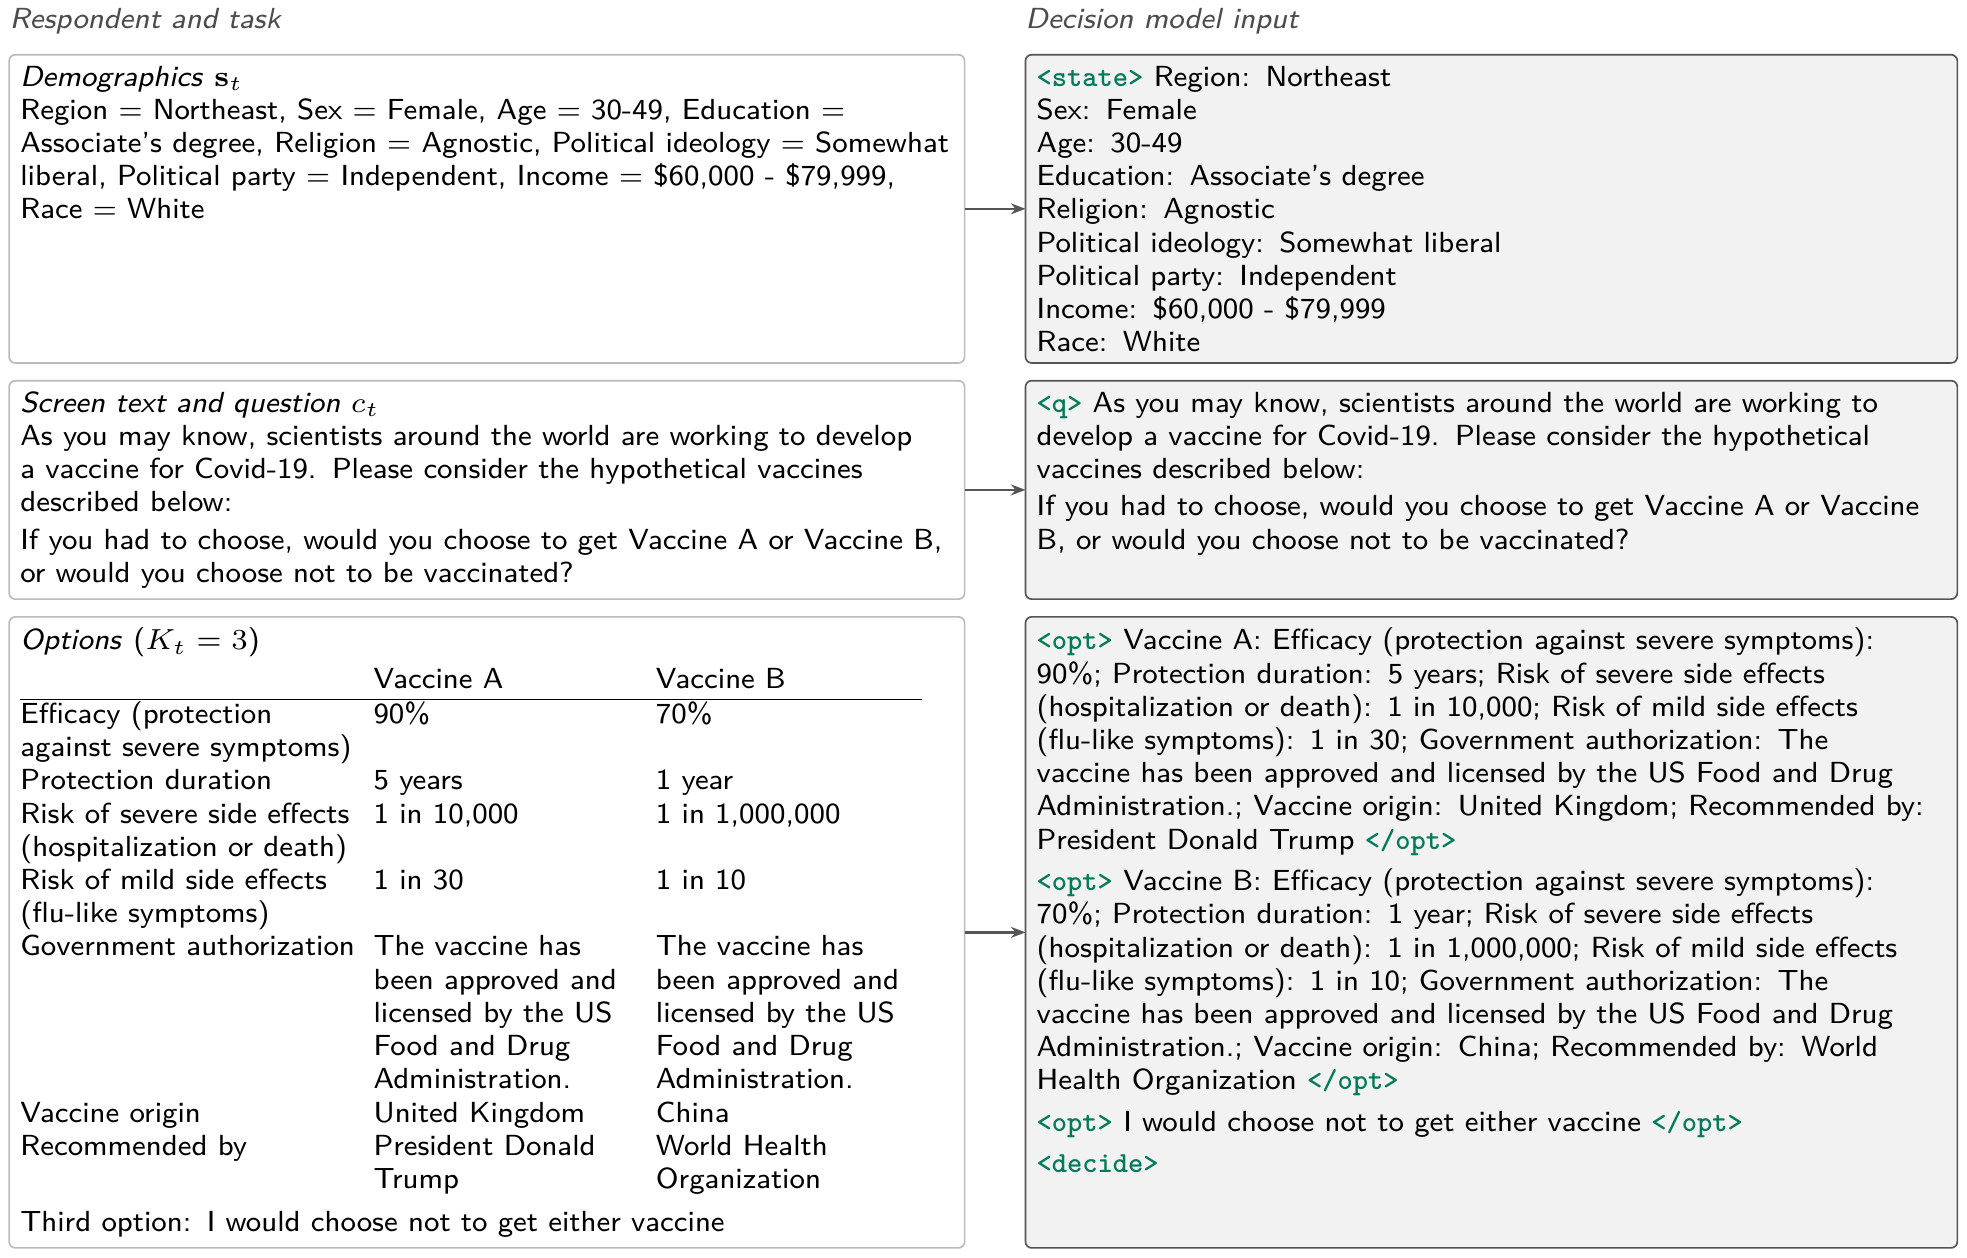
\includegraphics[width=1\linewidth,height=\textheight,keepaspectratio]{diagrams-tikz/fig_input_vaccines.png}

}

\caption{\label{appfig-input-vaccines}Full decision model input for one
unseen-study task (Vaccines)}

\end{appfig}%

\subsection*{Off-the-shelf generative LLM baseline
protocol}\label{off-the-shelf-generative-llm-baseline-protocol}
\addcontentsline{toc}{subsection}{Off-the-shelf generative LLM baseline
protocol}

\begin{tcolorbox}[enhanced jigsaw, arc=.35mm, bottomrule=.15mm, bottomtitle=1mm, breakable, colback=white, colbacktitle=quarto-callout-note-color!10!white, colframe=quarto-callout-note-color-frame, coltitle=black, left=2mm, leftrule=.75mm, opacityback=0, opacitybacktitle=0.6, rightrule=.15mm, title=\textcolor{quarto-callout-note-color}{\faInfo}\hspace{0.5em}{Note}, titlerule=0mm, toprule=.15mm, toptitle=1mm]

\textbf{TODO.} Add the generative LLM prompting protocol backing
Figure~\ref{fig-intro-off-the-shelf} and
\quartoapptblref{apptbl-llm-baseline}.

\end{tcolorbox}

\nexttablesize{\footnotesize}
{\def\LTcaptype{apptbl}
\begin{longtable}[]{@{}
  >{\raggedright\arraybackslash}p{(\linewidth - 14\tabcolsep) * \real{0.2215}}
  >{\raggedright\arraybackslash}p{(\linewidth - 14\tabcolsep) * \real{0.1456}}
  >{\raggedleft\arraybackslash}p{(\linewidth - 14\tabcolsep) * \real{0.1013}}
  >{\raggedleft\arraybackslash}p{(\linewidth - 14\tabcolsep) * \real{0.0886}}
  >{\raggedleft\arraybackslash}p{(\linewidth - 14\tabcolsep) * \real{0.1308}}
  >{\raggedleft\arraybackslash}p{(\linewidth - 14\tabcolsep) * \real{0.0759}}
  >{\raggedleft\arraybackslash}p{(\linewidth - 14\tabcolsep) * \real{0.1350}}
  >{\raggedleft\arraybackslash}p{(\linewidth - 14\tabcolsep) * \real{0.1013}}@{}}
\caption{{\label{apptbl-llm-baseline}}Off-the-shelf generative LLMs and
decision models on the 200-respondent Vaccines subsample}\tabularnewline
\toprule\noalign{}
\begin{minipage}[b]{\linewidth}\raggedright
Model
\end{minipage} & \begin{minipage}[b]{\linewidth}\raggedright
Reasoning effort
\end{minipage} & \begin{minipage}[b]{\linewidth}\raggedleft
Refusals
\end{minipage} & \begin{minipage}[b]{\linewidth}\raggedleft
Opt-out
\end{minipage} & \begin{minipage}[b]{\linewidth}\raggedleft
\(\mathrm{MSE}_\beta\) \(\times 10^3\)
\end{minipage} & \begin{minipage}[b]{\linewidth}\raggedleft
MAE
\end{minipage} & \begin{minipage}[b]{\linewidth}\raggedleft
Spearman \(\rho\)
\end{minipage} & \begin{minipage}[b]{\linewidth}\raggedleft
Sign acc.
\end{minipage} \\
\midrule\noalign{}
\endfirsthead
\toprule\noalign{}
\begin{minipage}[b]{\linewidth}\raggedright
Model
\end{minipage} & \begin{minipage}[b]{\linewidth}\raggedright
Reasoning effort
\end{minipage} & \begin{minipage}[b]{\linewidth}\raggedleft
Refusals
\end{minipage} & \begin{minipage}[b]{\linewidth}\raggedleft
Opt-out
\end{minipage} & \begin{minipage}[b]{\linewidth}\raggedleft
\(\mathrm{MSE}_\beta\) \(\times 10^3\)
\end{minipage} & \begin{minipage}[b]{\linewidth}\raggedleft
MAE
\end{minipage} & \begin{minipage}[b]{\linewidth}\raggedleft
Spearman \(\rho\)
\end{minipage} & \begin{minipage}[b]{\linewidth}\raggedleft
Sign acc.
\end{minipage} \\
\midrule\noalign{}
\endhead
\bottomrule\noalign{}
\endlastfoot
Human subsample (200 resp.) & Observed & 0 & 20.3\% & 0.46 & 0.018 &
0.89 & 100.0\% \\
Qwen3.5-0.8B & Off & 0 & 59.0\% & 2.75 & 0.038 & 0.82 & 90.9\% \\
Qwen3.5-0.8B & On & 19 & 28.6\% & 13.82 & 0.095 & 0.87 & 90.9\% \\
Qwen3.5-4B & Off & 0 & 53.6\% & 1.94 & 0.029 & 0.95 & 90.9\% \\
Qwen3.5-4B & On & 0 & 4.8\% & 9.71 & 0.085 & 0.98 & 100.0\% \\
Qwen3.5-9B & Off & 0 & 81.8\% & 1.49 & 0.027 & 0.95 & 90.9\% \\
Qwen3.5-9B & On & 1 & 11.4\% & 6.27 & 0.066 & 0.97 & 100.0\% \\
Gemini 3.5 Flash-Lite & Min & 0 & 21.9\% & 10.64 & 0.083 & 0.94 &
100.0\% \\
Gemini 3.5 Flash-Lite & High & 0 & 4.8\% & 12.28 & 0.085 & 0.90 &
100.0\% \\
Gemini 4 Argon & Low & 0 & 12.2\% & 16.50 & 0.099 & 0.93 & 100.0\% \\
Gemini 4 Argon & High & 0 & 9.1\% & 16.57 & 0.099 & 0.95 & 100.0\% \\
KEV-0.8B & Off-the-shelf & 0 & 32.1\% & 5.85 & 0.065 & 0.50 & 72.7\% \\
KEV-4B & Off-the-shelf & 0 & 13.4\% & 2.77 & 0.037 & 0.88 & 100.0\% \\
KEV-9B & Off-the-shelf & 0 & 16.3\% & 4.38 & 0.049 & 0.93 & 100.0\% \\
\end{longtable}
}

\emph{Note.} All models condition on respondent demographics over the
same 200-respondent, 1,000-task subsample of \texttt{Vaccines} (Kreps et
al. 2020), evaluated against the full-sample human OLS benchmark
(\(N = 1,971\)). Refusals count tasks where a generative LLM failed to
return a valid choice option. Opt-out reports the share (or expected
probability for decision models) of selecting neither vaccine. Values
back Figure~\ref{fig-intro-off-the-shelf}.

\subsection*{Attribute-level treatment-effect tables and
diagnostics}\label{attribute-level-treatment-effect-tables-and-diagnostics}
\addcontentsline{toc}{subsection}{Attribute-level treatment-effect
tables and diagnostics}

\begin{appfig}

\centering{

\includegraphics[width=1\linewidth,height=\textheight,keepaspectratio]{manuscript-training-assets/appfig-flights-slopes.png}

}

\caption{\label{appfig-flights-slopes}Flights (validation) OLS treatment
effects by attribute for off-the-shelf and pooled choice-trained models}

\end{appfig}%

\nexttablesize{\scriptsize}
{\def\LTcaptype{apptbl}
\begin{longtable}[]{@{}
  >{\raggedright\arraybackslash}p{(\linewidth - 14\tabcolsep) * \real{0.2700}}
  >{\raggedleft\arraybackslash}p{(\linewidth - 14\tabcolsep) * \real{0.0907}}
  >{\raggedleft\arraybackslash}p{(\linewidth - 14\tabcolsep) * \real{0.1076}}
  >{\raggedleft\arraybackslash}p{(\linewidth - 14\tabcolsep) * \real{0.1224}}
  >{\raggedleft\arraybackslash}p{(\linewidth - 14\tabcolsep) * \real{0.0949}}
  >{\raggedleft\arraybackslash}p{(\linewidth - 14\tabcolsep) * \real{0.1097}}
  >{\raggedleft\arraybackslash}p{(\linewidth - 14\tabcolsep) * \real{0.0949}}
  >{\raggedleft\arraybackslash}p{(\linewidth - 14\tabcolsep) * \real{0.1097}}@{}}
\caption{{\label{apptbl-vaccines-slopes}}Vaccines (held-out test) OLS
treatment effects by attribute}\tabularnewline
\toprule\noalign{}
\begin{minipage}[b]{\linewidth}\raggedright
Vaccine attribute level
\end{minipage} & \begin{minipage}[b]{\linewidth}\raggedleft
Human
\end{minipage} & \begin{minipage}[b]{\linewidth}\raggedleft
0.8B Base
\end{minipage} & \begin{minipage}[b]{\linewidth}\raggedleft
0.8B Pooled
\end{minipage} & \begin{minipage}[b]{\linewidth}\raggedleft
4B Base
\end{minipage} & \begin{minipage}[b]{\linewidth}\raggedleft
4B Pooled
\end{minipage} & \begin{minipage}[b]{\linewidth}\raggedleft
9B Base
\end{minipage} & \begin{minipage}[b]{\linewidth}\raggedleft
9B Pooled
\end{minipage} \\
\midrule\noalign{}
\endfirsthead
\toprule\noalign{}
\begin{minipage}[b]{\linewidth}\raggedright
Vaccine attribute level
\end{minipage} & \begin{minipage}[b]{\linewidth}\raggedleft
Human
\end{minipage} & \begin{minipage}[b]{\linewidth}\raggedleft
0.8B Base
\end{minipage} & \begin{minipage}[b]{\linewidth}\raggedleft
0.8B Pooled
\end{minipage} & \begin{minipage}[b]{\linewidth}\raggedleft
4B Base
\end{minipage} & \begin{minipage}[b]{\linewidth}\raggedleft
4B Pooled
\end{minipage} & \begin{minipage}[b]{\linewidth}\raggedleft
9B Base
\end{minipage} & \begin{minipage}[b]{\linewidth}\raggedleft
9B Pooled
\end{minipage} \\
\midrule\noalign{}
\endhead
\bottomrule\noalign{}
\endlastfoot
Efficacy: 70\% vs 50\% & 0.074 & 0.042 & 0.056 & 0.125 & 0.109 & 0.211 &
0.154 \\
Efficacy: 90\% vs 50\% & 0.164 & 0.065 & 0.104 & 0.238 & 0.211 & 0.369 &
0.289 \\
Duration: 5y vs 1y & 0.054 & 0.017 & 0.023 & 0.005 & 0.038 & 0.025 &
0.046 \\
Severe side effects: 1/1M vs 1/10k & 0.065 & 0.009 & 0.024 & 0.024 &
0.045 & 0.050 & 0.054 \\
Mild side effects: 1/30 vs 1/10 & 0.012 & -0.000 & -0.009 & 0.008 &
0.018 & 0.016 & 0.020 \\
FDA: EUA vs Full approval & -0.029 & 0.034 & 0.017 & -0.068 & -0.039 &
-0.008 & -0.013 \\
Origin: UK vs US & -0.038 & -0.025 & -0.030 & -0.081 & -0.053 & -0.072 &
-0.051 \\
Origin: China vs US & -0.131 & 0.028 & -0.004 & -0.197 & -0.114 & -0.205
& -0.143 \\
Endorsed: Biden vs Trump & 0.018 & 0.109 & 0.063 & 0.050 & 0.046 & 0.118
& 0.040 \\
Endorsed: CDC vs Trump & 0.089 & 0.273 & 0.081 & 0.284 & 0.138 & 0.306 &
0.123 \\
Endorsed: WHO vs Trump & 0.057 & 0.271 & 0.082 & 0.259 & 0.123 & 0.234 &
0.104 \\
\textbf{\(\mathrm{MSE}_\beta \times 10^3\)} & 0.00 & \textbf{12.07} &
\textbf{2.56} & \textbf{9.08} & \textbf{1.12} & \textbf{14.30} &
\textbf{2.43} \\
\end{longtable}
}

\emph{Note.} Human reports full-sample OLS slopes on observed respondent
choices in \texttt{Vaccines} (Kreps et al. 2020). Base denotes the
off-the-shelf decision model; Pooled denotes choice training on
\texttt{Drones\ +\ Electricity}. Values back
Figure~\ref{fig-results-vaccines-slopes}.

\nexttablesize{\scriptsize}
{\def\LTcaptype{apptbl}
\begin{longtable}[]{@{}
  >{\raggedright\arraybackslash}p{(\linewidth - 14\tabcolsep) * \real{0.2851}}
  >{\raggedleft\arraybackslash}p{(\linewidth - 14\tabcolsep) * \real{0.0901}}
  >{\raggedleft\arraybackslash}p{(\linewidth - 14\tabcolsep) * \real{0.1048}}
  >{\raggedleft\arraybackslash}p{(\linewidth - 14\tabcolsep) * \real{0.1174}}
  >{\raggedleft\arraybackslash}p{(\linewidth - 14\tabcolsep) * \real{0.0943}}
  >{\raggedleft\arraybackslash}p{(\linewidth - 14\tabcolsep) * \real{0.1069}}
  >{\raggedleft\arraybackslash}p{(\linewidth - 14\tabcolsep) * \real{0.0943}}
  >{\raggedleft\arraybackslash}p{(\linewidth - 14\tabcolsep) * \real{0.1069}}@{}}
\caption{{\label{apptbl-food-slopes}}Food labels (held-out test) OLS
treatment effects by arm}\tabularnewline
\toprule\noalign{}
\begin{minipage}[b]{\linewidth}\raggedright
Warning-label arm
\end{minipage} & \begin{minipage}[b]{\linewidth}\raggedleft
Human
\end{minipage} & \begin{minipage}[b]{\linewidth}\raggedleft
0.8B Base
\end{minipage} & \begin{minipage}[b]{\linewidth}\raggedleft
0.8B Pooled
\end{minipage} & \begin{minipage}[b]{\linewidth}\raggedleft
4B Base
\end{minipage} & \begin{minipage}[b]{\linewidth}\raggedleft
4B Pooled
\end{minipage} & \begin{minipage}[b]{\linewidth}\raggedleft
9B Base
\end{minipage} & \begin{minipage}[b]{\linewidth}\raggedleft
9B Pooled
\end{minipage} \\
\midrule\noalign{}
\endfirsthead
\toprule\noalign{}
\begin{minipage}[b]{\linewidth}\raggedright
Warning-label arm
\end{minipage} & \begin{minipage}[b]{\linewidth}\raggedleft
Human
\end{minipage} & \begin{minipage}[b]{\linewidth}\raggedleft
0.8B Base
\end{minipage} & \begin{minipage}[b]{\linewidth}\raggedleft
0.8B Pooled
\end{minipage} & \begin{minipage}[b]{\linewidth}\raggedleft
4B Base
\end{minipage} & \begin{minipage}[b]{\linewidth}\raggedleft
4B Pooled
\end{minipage} & \begin{minipage}[b]{\linewidth}\raggedleft
9B Base
\end{minipage} & \begin{minipage}[b]{\linewidth}\raggedleft
9B Pooled
\end{minipage} \\
\midrule\noalign{}
\endhead
\bottomrule\noalign{}
\endlastfoot
NutritionInfo vs Positive & 0.184 & 0.128 & 0.161 & 0.250 & 0.199 &
0.358 & 0.344 \\
HighIn vs Positive & 0.054 & 0.123 & 0.076 & -0.208 & -0.020 & -0.124 &
-0.005 \\
Positive+NutritionInfo vs Positive & 0.179 & 0.157 & 0.167 & 0.305 &
0.183 & 0.370 & 0.331 \\
Positive+HighIn vs Positive & 0.119 & -0.008 & 0.023 & -0.002 & 0.047 &
0.019 & 0.192 \\
Spectrum vs Positive & 0.108 & 0.057 & 0.074 & 0.067 & 0.128 & 0.179 &
0.239 \\
\textbf{\(\mathrm{MSE}_\beta \times 10^3\)} & 0.00 & \textbf{5.46} &
\textbf{2.30} & \textbf{21.10} & \textbf{2.28} & \textbf{22.73} &
\textbf{14.82} \\
\end{longtable}
}

\emph{Note.} Human reports full-sample OLS slopes on observed choices in
\texttt{Food\ labels} (Grummon et al. 2025). Base denotes the
off-the-shelf decision model; Pooled denotes choice training on
\texttt{Drones\ +\ Electricity}.

\nexttablesize{\scriptsize}
{\def\LTcaptype{apptbl}
\begin{longtable}[]{@{}
  >{\raggedright\arraybackslash}p{(\linewidth - 14\tabcolsep) * \real{0.3249}}
  >{\raggedleft\arraybackslash}p{(\linewidth - 14\tabcolsep) * \real{0.0901}}
  >{\raggedleft\arraybackslash}p{(\linewidth - 14\tabcolsep) * \real{0.0964}}
  >{\raggedleft\arraybackslash}p{(\linewidth - 14\tabcolsep) * \real{0.1069}}
  >{\raggedleft\arraybackslash}p{(\linewidth - 14\tabcolsep) * \real{0.0901}}
  >{\raggedleft\arraybackslash}p{(\linewidth - 14\tabcolsep) * \real{0.1006}}
  >{\raggedleft\arraybackslash}p{(\linewidth - 14\tabcolsep) * \real{0.0901}}
  >{\raggedleft\arraybackslash}p{(\linewidth - 14\tabcolsep) * \real{0.1006}}@{}}
\caption{{\label{apptbl-consumer-rights-slopes}}Consumer rights
(held-out test) OLS treatment effects by attribute}\tabularnewline
\toprule\noalign{}
\begin{minipage}[b]{\linewidth}\raggedright
Product and attribute level
\end{minipage} & \begin{minipage}[b]{\linewidth}\raggedleft
Human
\end{minipage} & \begin{minipage}[b]{\linewidth}\raggedleft
0.8B Base
\end{minipage} & \begin{minipage}[b]{\linewidth}\raggedleft
0.8B Pooled
\end{minipage} & \begin{minipage}[b]{\linewidth}\raggedleft
4B Base
\end{minipage} & \begin{minipage}[b]{\linewidth}\raggedleft
4B Pooled
\end{minipage} & \begin{minipage}[b]{\linewidth}\raggedleft
9B Base
\end{minipage} & \begin{minipage}[b]{\linewidth}\raggedleft
9B Pooled
\end{minipage} \\
\midrule\noalign{}
\endfirsthead
\toprule\noalign{}
\begin{minipage}[b]{\linewidth}\raggedright
Product and attribute level
\end{minipage} & \begin{minipage}[b]{\linewidth}\raggedleft
Human
\end{minipage} & \begin{minipage}[b]{\linewidth}\raggedleft
0.8B Base
\end{minipage} & \begin{minipage}[b]{\linewidth}\raggedleft
0.8B Pooled
\end{minipage} & \begin{minipage}[b]{\linewidth}\raggedleft
4B Base
\end{minipage} & \begin{minipage}[b]{\linewidth}\raggedleft
4B Pooled
\end{minipage} & \begin{minipage}[b]{\linewidth}\raggedleft
9B Base
\end{minipage} & \begin{minipage}[b]{\linewidth}\raggedleft
9B Pooled
\end{minipage} \\
\midrule\noalign{}
\endhead
\bottomrule\noalign{}
\endlastfoot
Computers \textbar{} Price: \$1250 vs \$2000 & 0.097 & 0.003 & 0.000 &
0.037 & 0.079 & 0.113 & 0.150 \\
Computers \textbar{} Price: \$500 vs \$2000 & 0.220 & 0.011 & 0.026 &
0.027 & 0.128 & 0.154 & 0.259 \\
Computers \textbar{} Brand: Apple MacBook vs Medion & 0.031 & -0.012 &
0.014 & -0.023 & 0.020 & -0.058 & -0.017 \\
Computers \textbar{} Brand: Lenovo vs Medion & 0.046 & -0.006 & 0.002 &
0.013 & 0.019 & -0.004 & 0.003 \\
Computers \textbar{} Brand: HP vs Medion & 0.080 & -0.001 & 0.001 &
0.012 & 0.019 & -0.015 & -0.007 \\
Computers \textbar{} RAM: 10 GB vs 4 GB & 0.092 & -0.001 & 0.018 & 0.012
& 0.046 & 0.093 & 0.116 \\
Computers \textbar{} RAM: 16 GB vs 4 GB & 0.147 & 0.008 & 0.036 & 0.045
& 0.085 & 0.152 & 0.193 \\
Computers \textbar{} Storage: 256 GB vs 128 GB & 0.063 & 0.000 & 0.002 &
0.031 & 0.040 & 0.055 & 0.072 \\
Computers \textbar{} Storage: 512 GB vs 128 GB & 0.119 & -0.009 & 0.007
& 0.046 & 0.073 & 0.092 & 0.135 \\
Computers \textbar{} Processor: AMD vs Qualcomm snapdragon & 0.002 &
0.014 & -0.006 & 0.028 & 0.015 & 0.032 & 0.018 \\
Computers \textbar{} Processor: Intel vs Qualcomm snapdragon & 0.030 &
0.014 & -0.003 & 0.026 & 0.012 & 0.037 & 0.017 \\
Computers \textbar{} Warranty: 1 year vs No warranty & 0.080 & 0.008 &
0.010 & 0.049 & 0.044 & 0.047 & 0.053 \\
Computers \textbar{} Warranty: 10 years vs No warranty & 0.169 & 0.003 &
0.027 & 0.051 & 0.077 & 0.057 & 0.106 \\
Computers \textbar{} Privacy: No privacy (marketing) vs No privacy &
-0.026 & -0.003 & -0.012 & -0.028 & -0.013 & -0.025 & -0.011 \\
Computers \textbar{} Privacy: No privacy (sustainability) vs No privacy
& -0.004 & -0.003 & -0.002 & -0.022 & 0.013 & -0.018 & 0.006 \\
Computers \textbar{} Privacy: Full privacy vs No privacy & 0.016 & 0.003
& 0.012 & -0.004 & 0.054 & -0.008 & 0.028 \\
Computers \textbar{} Liability: Seller and consumer vs The consumer &
0.019 & -0.003 & 0.006 & -0.001 & 0.020 & 0.016 & 0.050 \\
Computers \textbar{} Liability: The seller vs The consumer & 0.024 &
0.003 & 0.003 & 0.005 & 0.031 & 0.035 & 0.046 \\
Computers \textbar{} Conflict resolution: The consumer vs The seller &
0.009 & 0.047 & 0.029 & -0.029 & 0.021 & 0.031 & 0.044 \\
Laundry \textbar{} Price: \$900 vs \$1400 & 0.113 & 0.012 & 0.045 &
0.035 & 0.072 & 0.097 & 0.132 \\
Laundry \textbar{} Price: \$400 vs \$1400 & 0.215 & 0.011 & 0.092 &
0.056 & 0.127 & 0.179 & 0.269 \\
Laundry \textbar{} Brand: Hoover vs Haier & 0.018 & -0.010 & -0.015 &
0.004 & 0.004 & -0.006 & 0.002 \\
Laundry \textbar{} Brand: General Electric vs Haier & 0.043 & 0.002 &
-0.014 & 0.007 & 0.008 & 0.011 & 0.008 \\
Laundry \textbar{} Brand: Whirlpool vs Haier & 0.061 & 0.000 & -0.009 &
0.011 & 0.009 & 0.011 & 0.010 \\
Laundry \textbar{} Depth: 32 inches vs 28 inches & 0.033 & 0.001 & 0.006
& -0.002 & -0.002 & -0.010 & -0.008 \\
Laundry \textbar{} Depth: 36 inches vs 28 inches & 0.055 & -0.001 &
0.008 & -0.004 & -0.004 & -0.015 & -0.015 \\
Laundry \textbar{} Noise: 75 dB vs 78 dB & 0.005 & -0.013 & 0.006 &
0.004 & 0.022 & 0.019 & 0.035 \\
Laundry \textbar{} Noise: 70 dB vs 78 dB & 0.019 & -0.010 & 0.021 &
0.018 & 0.050 & 0.046 & 0.079 \\
Laundry \textbar{} Load capacity: 12 pounds vs 6 pounds & 0.096 & 0.005
& 0.009 & 0.041 & 0.055 & 0.105 & 0.114 \\
Laundry \textbar{} Load capacity: 20 pounds vs 6 pounds & 0.170 & -0.005
& 0.016 & 0.067 & 0.092 & 0.150 & 0.181 \\
Laundry \textbar{} Warranty: 1 year vs No warranty & 0.103 & -0.006 &
0.009 & 0.043 & 0.040 & 0.065 & 0.071 \\
Laundry \textbar{} Warranty: 10 years vs No warranty & 0.227 & -0.003 &
0.029 & 0.065 & 0.092 & 0.134 & 0.171 \\
Laundry \textbar{} Privacy: No privacy (marketing) vs No privacy &
-0.013 & 0.008 & -0.004 & -0.037 & -0.006 & -0.017 & -0.005 \\
Laundry \textbar{} Privacy: No privacy (sustainability) vs No privacy &
0.010 & 0.003 & 0.006 & -0.022 & 0.019 & -0.018 & 0.005 \\
Laundry \textbar{} Privacy: Full privacy vs No privacy & 0.022 & 0.026 &
-0.003 & -0.011 & 0.049 & -0.008 & 0.026 \\
Laundry \textbar{} Liability: Seller and consumer vs The consumer &
0.024 & 0.012 & 0.014 & -0.019 & 0.004 & 0.006 & 0.048 \\
Laundry \textbar{} Liability: The seller vs The consumer & 0.033 & 0.020
& 0.009 & -0.019 & 0.017 & 0.025 & 0.043 \\
Laundry \textbar{} Conflict resolution: The consumer vs The seller &
0.020 & 0.055 & 0.034 & -0.040 & 0.015 & 0.025 & 0.043 \\
\textbf{Price \(\mathrm{MSE}_\beta \times 10^3\) (4)} & 0.00 &
\textbf{26.02} & \textbf{16.64} & \textbf{18.12} & \textbf{4.54} &
\textbf{1.53} & \textbf{1.91} \\
\textbf{Non-price \(\mathrm{MSE}_\beta \times 10^3\) (34)} & 0.00 &
\textbf{6.26} & \textbf{4.79} & \textbf{3.33} & \textbf{1.98} &
\textbf{1.79} & \textbf{1.29} \\
\textbf{Overall \(\mathrm{MSE}_\beta \times 10^3\) (38)} & 0.00 &
\textbf{8.34} & \textbf{6.04} & \textbf{4.89} & \textbf{2.25} &
\textbf{1.76} & \textbf{1.36} \\
\end{longtable}
}

\emph{Note.} Human reports full-sample OLS slopes across the 19 laptop
(\texttt{Computers}) and 19 laundry-machine (\texttt{Laundry}) attribute
levels in \texttt{Consumer\ rights} (Kantorowicz-Reznichenko et al.
2026). Base denotes the off-the-shelf decision model; Pooled denotes
choice training on \texttt{Drones\ +\ Electricity}. Laptop slopes back
Figure~\ref{fig-results-laptops-slopes}.

\nexttablesize{\scriptsize}
{\def\LTcaptype{apptbl}
\begin{longtable}[]{@{}
  >{\raggedright\arraybackslash}p{(\linewidth - 14\tabcolsep) * \real{0.3095}}
  >{\raggedleft\arraybackslash}p{(\linewidth - 14\tabcolsep) * \real{0.0905}}
  >{\raggedleft\arraybackslash}p{(\linewidth - 14\tabcolsep) * \real{0.0989}}
  >{\raggedleft\arraybackslash}p{(\linewidth - 14\tabcolsep) * \real{0.1095}}
  >{\raggedleft\arraybackslash}p{(\linewidth - 14\tabcolsep) * \real{0.0926}}
  >{\raggedleft\arraybackslash}p{(\linewidth - 14\tabcolsep) * \real{0.1032}}
  >{\raggedleft\arraybackslash}p{(\linewidth - 14\tabcolsep) * \real{0.0926}}
  >{\raggedleft\arraybackslash}p{(\linewidth - 14\tabcolsep) * \real{0.1032}}@{}}
\caption{{\label{apptbl-ai-offshoring-slopes}}AI \& offshoring
(held-out test) OLS treatment effects by attribute}\tabularnewline
\toprule\noalign{}
\begin{minipage}[b]{\linewidth}\raggedright
Country, arm, and attribute level
\end{minipage} & \begin{minipage}[b]{\linewidth}\raggedleft
Human
\end{minipage} & \begin{minipage}[b]{\linewidth}\raggedleft
0.8B Base
\end{minipage} & \begin{minipage}[b]{\linewidth}\raggedleft
0.8B Pooled
\end{minipage} & \begin{minipage}[b]{\linewidth}\raggedleft
4B Base
\end{minipage} & \begin{minipage}[b]{\linewidth}\raggedleft
4B Pooled
\end{minipage} & \begin{minipage}[b]{\linewidth}\raggedleft
9B Base
\end{minipage} & \begin{minipage}[b]{\linewidth}\raggedleft
9B Pooled
\end{minipage} \\
\midrule\noalign{}
\endfirsthead
\toprule\noalign{}
\begin{minipage}[b]{\linewidth}\raggedright
Country, arm, and attribute level
\end{minipage} & \begin{minipage}[b]{\linewidth}\raggedleft
Human
\end{minipage} & \begin{minipage}[b]{\linewidth}\raggedleft
0.8B Base
\end{minipage} & \begin{minipage}[b]{\linewidth}\raggedleft
0.8B Pooled
\end{minipage} & \begin{minipage}[b]{\linewidth}\raggedleft
4B Base
\end{minipage} & \begin{minipage}[b]{\linewidth}\raggedleft
4B Pooled
\end{minipage} & \begin{minipage}[b]{\linewidth}\raggedleft
9B Base
\end{minipage} & \begin{minipage}[b]{\linewidth}\raggedleft
9B Pooled
\end{minipage} \\
\midrule\noalign{}
\endhead
\bottomrule\noalign{}
\endlastfoot
US AI \textbar{} Price: \$450 vs \$600 & 0.313 & -0.002 & 0.031 & 0.105
& 0.171 & 0.236 & 0.331 \\
US AI \textbar{} Price: \$300 vs \$600 & 0.351 & -0.013 & 0.022 & 0.174
& 0.242 & 0.256 & 0.364 \\
US AI \textbar{} Customer service jobs: 75 vs 100 & -0.197 & -0.010 &
-0.054 & -0.296 & -0.251 & -0.121 & -0.154 \\
US AI \textbar{} Customer service jobs: 125 vs 100 & 0.072 & 0.037 &
0.061 & 0.394 & 0.294 & 0.172 & 0.153 \\
US AI \textbar{} Factory jobs: 300 vs 400 & -0.389 & -0.078 & -0.125 &
-0.502 & -0.590 & -0.511 & -0.613 \\
US AI \textbar{} Factory jobs: 500 vs 400 & 0.140 & 0.028 & 0.072 &
0.800 & 0.638 & 0.841 & 0.636 \\
US AI \textbar{} Data science jobs: 150 vs 200 & -0.215 & -0.055 &
-0.087 & -0.408 & -0.376 & -0.258 & -0.347 \\
US AI \textbar{} Data science jobs: 250 vs 200 & 0.075 & 0.109 & 0.160 &
0.329 & 0.248 & 0.020 & -0.001 \\
US Offshoring \textbar{} Price: \$450 vs \$600 & 0.227 & 0.005 & 0.016 &
0.141 & 0.186 & 0.414 & 0.522 \\
US Offshoring \textbar{} Price: \$300 vs \$600 & 0.261 & -0.032 & -0.023
& 0.159 & 0.214 & 0.466 & 0.587 \\
US Offshoring \textbar{} Customer service jobs: 75 vs 100 & -0.185 &
-0.010 & -0.059 & -0.351 & -0.249 & -0.145 & -0.146 \\
US Offshoring \textbar{} Customer service jobs: 125 vs 100 & 0.108 &
0.045 & 0.062 & 0.352 & 0.242 & 0.207 & 0.194 \\
US Offshoring \textbar{} Factory jobs: 300 vs 400 & -0.308 & -0.038 &
-0.091 & -0.442 & -0.495 & -0.509 & -0.552 \\
US Offshoring \textbar{} Factory jobs: 500 vs 400 & 0.081 & 0.067 &
0.115 & 0.787 & 0.652 & 0.800 & 0.576 \\
US Offshoring \textbar{} Data science jobs: 150 vs 200 & -0.128 & -0.015
& -0.069 & -0.297 & -0.273 & -0.262 & -0.307 \\
US Offshoring \textbar{} Data science jobs: 250 vs 200 & 0.087 & 0.142 &
0.199 & 0.422 & 0.333 & 0.069 & 0.071 \\
Canada AI \textbar{} Price: \$450 vs \$600 & 0.209 & -0.005 & 0.022 &
0.118 & 0.163 & 0.214 & 0.303 \\
Canada AI \textbar{} Price: \$300 vs \$600 & 0.263 & -0.020 & 0.007 &
0.163 & 0.219 & 0.225 & 0.322 \\
Canada AI \textbar{} Customer service jobs: 75 vs 100 & -0.188 & -0.015
& -0.060 & -0.297 & -0.240 & -0.116 & -0.166 \\
Canada AI \textbar{} Customer service jobs: 125 vs 100 & 0.036 & 0.038 &
0.067 & 0.339 & 0.281 & 0.149 & 0.139 \\
Canada AI \textbar{} Factory jobs: 300 vs 400 & -0.251 & -0.076 & -0.132
& -0.490 & -0.567 & -0.488 & -0.608 \\
Canada AI \textbar{} Factory jobs: 500 vs 400 & 0.111 & 0.036 & 0.083 &
0.769 & 0.649 & 0.841 & 0.650 \\
Canada AI \textbar{} Data science jobs: 150 vs 200 & -0.069 & -0.049 &
-0.084 & -0.410 & -0.356 & -0.236 & -0.321 \\
Canada AI \textbar{} Data science jobs: 250 vs 200 & 0.077 & 0.112 &
0.165 & 0.292 & 0.230 & -0.005 & -0.028 \\
Canada Offshoring \textbar{} Price: \$450 vs \$600 & 0.195 & 0.006 &
0.011 & 0.139 & 0.171 & 0.394 & 0.493 \\
Canada Offshoring \textbar{} Price: \$300 vs \$600 & 0.274 & -0.029 &
-0.027 & 0.154 & 0.207 & 0.468 & 0.606 \\
Canada Offshoring \textbar{} Customer service jobs: 75 vs 100 & -0.156 &
-0.013 & -0.063 & -0.334 & -0.244 & -0.136 & -0.148 \\
Canada Offshoring \textbar{} Customer service jobs: 125 vs 100 & 0.009 &
0.040 & 0.066 & 0.346 & 0.243 & 0.229 & 0.215 \\
Canada Offshoring \textbar{} Factory jobs: 300 vs 400 & -0.264 & -0.036
& -0.094 & -0.404 & -0.476 & -0.493 & -0.527 \\
Canada Offshoring \textbar{} Factory jobs: 500 vs 400 & 0.050 & 0.069 &
0.122 & 0.806 & 0.682 & 0.836 & 0.622 \\
Canada Offshoring \textbar{} Data science jobs: 150 vs 200 & -0.164 &
-0.012 & -0.068 & -0.304 & -0.269 & -0.233 & -0.260 \\
Canada Offshoring \textbar{} Data science jobs: 250 vs 200 & 0.073 &
0.135 & 0.200 & 0.417 & 0.325 & 0.105 & 0.090 \\
\textbf{Price \(\mathrm{MSE}_\beta \times 10^3\) (8)} & 0.00 &
\textbf{77.60} & \textbf{67.37} & \textbf{16.09} & \textbf{5.66} &
\textbf{21.31} & \textbf{50.56} \\
\textbf{Non-price \(\mathrm{MSE}_\beta \times 10^3\) (24)} & 0.00 &
\textbf{19.36} & \textbf{13.03} & \textbf{126.66} & \textbf{83.42} &
\textbf{103.41} & \textbf{67.80} \\
\textbf{Overall \(\mathrm{MSE}_\beta \times 10^3\) (32)} & 0.00 &
\textbf{33.92} & \textbf{26.61} & \textbf{99.01} & \textbf{63.98} &
\textbf{82.89} & \textbf{63.49} \\
\end{longtable}
}

\emph{Note.} Human reports full-sample OLS slopes on the five-point
ordinal support scale across four country-by-arm regressions (8 slopes
each, 32 total) in \texttt{AI\ \&\ offshoring} (Magistro et al. 2026).
Base denotes the off-the-shelf decision model; Pooled denotes choice
training on \texttt{Drones\ +\ Electricity}.

\nexttablesize{\scriptsize}
{\def\LTcaptype{apptbl}
\begin{longtable}[]{@{}
  >{\raggedright\arraybackslash}p{(\linewidth - 14\tabcolsep) * \real{0.2647}}
  >{\raggedleft\arraybackslash}p{(\linewidth - 14\tabcolsep) * \real{0.0903}}
  >{\raggedleft\arraybackslash}p{(\linewidth - 14\tabcolsep) * \real{0.1071}}
  >{\raggedleft\arraybackslash}p{(\linewidth - 14\tabcolsep) * \real{0.1218}}
  >{\raggedleft\arraybackslash}p{(\linewidth - 14\tabcolsep) * \real{0.0966}}
  >{\raggedleft\arraybackslash}p{(\linewidth - 14\tabcolsep) * \real{0.1113}}
  >{\raggedleft\arraybackslash}p{(\linewidth - 14\tabcolsep) * \real{0.0966}}
  >{\raggedleft\arraybackslash}p{(\linewidth - 14\tabcolsep) * \real{0.1113}}@{}}
\caption{{\label{apptbl-flights-slopes}}Flights (validation) OLS
treatment effects by attribute}\tabularnewline
\toprule\noalign{}
\begin{minipage}[b]{\linewidth}\raggedright
Flight attribute level
\end{minipage} & \begin{minipage}[b]{\linewidth}\raggedleft
Human
\end{minipage} & \begin{minipage}[b]{\linewidth}\raggedleft
0.8B Base
\end{minipage} & \begin{minipage}[b]{\linewidth}\raggedleft
0.8B Pooled
\end{minipage} & \begin{minipage}[b]{\linewidth}\raggedleft
4B Base
\end{minipage} & \begin{minipage}[b]{\linewidth}\raggedleft
4B Pooled
\end{minipage} & \begin{minipage}[b]{\linewidth}\raggedleft
9B Base
\end{minipage} & \begin{minipage}[b]{\linewidth}\raggedleft
9B Pooled
\end{minipage} \\
\midrule\noalign{}
\endfirsthead
\toprule\noalign{}
\begin{minipage}[b]{\linewidth}\raggedright
Flight attribute level
\end{minipage} & \begin{minipage}[b]{\linewidth}\raggedleft
Human
\end{minipage} & \begin{minipage}[b]{\linewidth}\raggedleft
0.8B Base
\end{minipage} & \begin{minipage}[b]{\linewidth}\raggedleft
0.8B Pooled
\end{minipage} & \begin{minipage}[b]{\linewidth}\raggedleft
4B Base
\end{minipage} & \begin{minipage}[b]{\linewidth}\raggedleft
4B Pooled
\end{minipage} & \begin{minipage}[b]{\linewidth}\raggedleft
9B Base
\end{minipage} & \begin{minipage}[b]{\linewidth}\raggedleft
9B Pooled
\end{minipage} \\
\midrule\noalign{}
\endhead
\bottomrule\noalign{}
\endlastfoot
Price: \$275 & -0.085 & 0.003 & -0.070 & -0.055 & -0.088 & -0.027 &
-0.068 \\
Price: \$300 & -0.195 & -0.013 & -0.152 & -0.101 & -0.186 & -0.064 &
-0.172 \\
Price: \$325 & -0.304 & -0.020 & -0.233 & -0.164 & -0.280 & -0.127 &
-0.264 \\
Fuel: Sustainable aviation fuel & 0.069 & -0.057 & 0.010 & 0.100 & 0.079
& 0.026 & 0.049 \\
Airline: Frontier & -0.085 & 0.034 & 0.006 & -0.180 & -0.089 & -0.127 &
-0.092 \\
Airline: Southwest & -0.024 & 0.027 & 0.003 & 0.022 & 0.012 & 0.021 &
0.036 \\
Airline: United & -0.022 & 0.001 & 0.002 & -0.016 & -0.010 & -0.013 &
-0.012 \\
Baggage: Checked bag+carry-on & 0.056 & -0.043 & -0.026 & 0.087 & 0.069
& 0.086 & 0.089 \\
Baggage: Personal item only & -0.139 & -0.003 & -0.014 & -0.186 & -0.092
& -0.120 & -0.103 \\
Space: Extra legroom & 0.065 & -0.081 & -0.003 & 0.124 & 0.114 & 0.043 &
0.088 \\
Seat: Middle & -0.091 & -0.006 & -0.004 & -0.084 & -0.061 & -0.065 &
-0.063 \\
Seat: Window & 0.038 & 0.009 & 0.009 & 0.009 & 0.008 & 0.004 & 0.008 \\
\textbf{\(\mathrm{MSE}_\beta \times 10^3\)} & 0.00 & \textbf{17.75} &
\textbf{4.62} & \textbf{4.10} & \textbf{0.73} & \textbf{5.12} &
\textbf{0.93} \\
\end{longtable}
}

\emph{Note.} Human reports full-sample OLS slopes on observed respondent
choices in \texttt{Flights} (Goldfarb et al. 2026), the validation
dataset used to select each run's checkpoint. Base denotes the
off-the-shelf decision model; Pooled denotes choice training on
\texttt{Drones\ +\ Electricity}. Values back
\quartoappfigref{appfig-flights-slopes}.

\nexttablesize{\scriptsize}
{\def\LTcaptype{apptbl}
\begin{longtable}[]{@{}
  >{\raggedright\arraybackslash}p{(\linewidth - 18\tabcolsep) * \real{0.1292}}
  >{\raggedleft\arraybackslash}p{(\linewidth - 18\tabcolsep) * \real{0.0899}}
  >{\raggedleft\arraybackslash}p{(\linewidth - 18\tabcolsep) * \real{0.0899}}
  >{\raggedleft\arraybackslash}p{(\linewidth - 18\tabcolsep) * \real{0.1011}}
  >{\raggedleft\arraybackslash}p{(\linewidth - 18\tabcolsep) * \real{0.0899}}
  >{\raggedleft\arraybackslash}p{(\linewidth - 18\tabcolsep) * \real{0.0955}}
  >{\raggedleft\arraybackslash}p{(\linewidth - 18\tabcolsep) * \real{0.0899}}
  >{\raggedleft\arraybackslash}p{(\linewidth - 18\tabcolsep) * \real{0.0955}}
  >{\raggedleft\arraybackslash}p{(\linewidth - 18\tabcolsep) * \real{0.0843}}
  >{\raggedleft\arraybackslash}p{(\linewidth - 18\tabcolsep) * \real{0.0899}}@{}}
\caption{{\label{apptbl-magistro-subsets}}AI \& offshoring OLS
treatment-effect error (\(\mathrm{MSE}_\beta \times 10^3\)) by country,
arm, and attribute type}\tabularnewline
\toprule\noalign{}
\begin{minipage}[b]{\linewidth}\raggedright
Trained on
\end{minipage} & \begin{minipage}[b]{\linewidth}\raggedleft
All (32)
\end{minipage} & \begin{minipage}[b]{\linewidth}\raggedleft
US (16)
\end{minipage} & \begin{minipage}[b]{\linewidth}\raggedleft
Canada (16)
\end{minipage} & \begin{minipage}[b]{\linewidth}\raggedleft
US AI (8)
\end{minipage} & \begin{minipage}[b]{\linewidth}\raggedleft
US Off. (8)
\end{minipage} & \begin{minipage}[b]{\linewidth}\raggedleft
CA AI (8)
\end{minipage} & \begin{minipage}[b]{\linewidth}\raggedleft
CA Off. (8)
\end{minipage} & \begin{minipage}[b]{\linewidth}\raggedleft
Price (8)
\end{minipage} & \begin{minipage}[b]{\linewidth}\raggedleft
Jobs (24)
\end{minipage} \\
\midrule\noalign{}
\endfirsthead
\toprule\noalign{}
\begin{minipage}[b]{\linewidth}\raggedright
Trained on
\end{minipage} & \begin{minipage}[b]{\linewidth}\raggedleft
All (32)
\end{minipage} & \begin{minipage}[b]{\linewidth}\raggedleft
US (16)
\end{minipage} & \begin{minipage}[b]{\linewidth}\raggedleft
Canada (16)
\end{minipage} & \begin{minipage}[b]{\linewidth}\raggedleft
US AI (8)
\end{minipage} & \begin{minipage}[b]{\linewidth}\raggedleft
US Off. (8)
\end{minipage} & \begin{minipage}[b]{\linewidth}\raggedleft
CA AI (8)
\end{minipage} & \begin{minipage}[b]{\linewidth}\raggedleft
CA Off. (8)
\end{minipage} & \begin{minipage}[b]{\linewidth}\raggedleft
Price (8)
\end{minipage} & \begin{minipage}[b]{\linewidth}\raggedleft
Jobs (24)
\end{minipage} \\
\midrule\noalign{}
\endhead
\bottomrule\noalign{}
\endlastfoot
\multicolumn{10}{@{}>{\centering\arraybackslash}p{(\linewidth - 18\tabcolsep) * \real{0.9551} + 18\tabcolsep}@{}}{%
\emph{KEV-0.8B}} \\
Off-the-shelf & 33.92 & 41.48 & 26.35 & 50.62 & 32.34 & 24.20 & 28.51 &
77.60 & 19.36 \\
Electricity & 29.60 & 35.59 & 23.62 & 42.21 & 28.96 & 20.16 & 27.08 &
71.71 & 15.57 \\
Drones & 34.41 & 41.14 & 27.67 & 49.82 & 32.46 & 25.25 & 30.10 & 83.27 &
18.12 \\
Drones + Electricity & \textbf{26.61} & \textbf{32.17} & \textbf{21.06}
& \textbf{38.38} & \textbf{25.96} & \textbf{17.60} & \textbf{24.51} &
\textbf{67.37} & \textbf{13.03} \\
\multicolumn{10}{@{}>{\centering\arraybackslash}p{(\linewidth - 18\tabcolsep) * \real{0.9551} + 18\tabcolsep}@{}}{%
\emph{KEV-4B}} \\
Off-the-shelf & 99.01 & 93.76 & 104.27 & 92.30 & 95.22 & 96.88 & 111.65
& 16.09 & 126.66 \\
Electricity & 113.26 & 106.45 & 120.08 & 101.87 & 111.03 & 112.91 &
127.26 & 11.67 & 147.13 \\
Drones & 74.69 & 67.29 & 82.09 & 60.96 & 73.62 & 74.73 & 89.45 & 6.21 &
97.52 \\
Drones + Electricity & \textbf{63.98} & \textbf{56.05} & \textbf{71.90}
& \textbf{53.45} & \textbf{58.66} & \textbf{70.30} & \textbf{73.49} &
\textbf{5.66} & \textbf{83.42} \\
\multicolumn{10}{@{}>{\centering\arraybackslash}p{(\linewidth - 18\tabcolsep) * \real{0.9551} + 18\tabcolsep}@{}}{%
\emph{KEV-9B}} \\
Off-the-shelf & 82.89 & 75.34 & 90.43 & 67.71 & 82.98 & 80.55 & 100.31 &
\textbf{21.31} & 103.41 \\
Electricity & 95.68 & 83.68 & 107.69 & 71.35 & 96.01 & 98.52 & 116.86 &
37.05 & 115.23 \\
Drones & 87.42 & 79.58 & 95.26 & 68.44 & 90.72 & 86.34 & 104.18 & 37.14
& 104.18 \\
Drones + Electricity & \textbf{63.49} & \textbf{54.14} & \textbf{72.83}
& \textbf{40.89} & \textbf{67.39} & \textbf{64.66} & \textbf{81.00} &
50.56 & \textbf{67.80} \\
\end{longtable}
}

\emph{Note.} Values report \(\mathrm{MSE}_\beta \times 10^3\) on
\texttt{AI\ \&\ offshoring} (Magistro et al. 2026); lower is better.
Bold marks the lowest value per model and subset. Pooled choice training
(\texttt{Drones\ +\ Electricity}) improves every country and arm subset
across all three models, whereas single-dataset training on
\texttt{Electricity} degrades both US and Canada subsets on
\texttt{KEV-4B} and \texttt{KEV-9B}.




\end{document}
